\begin{bibunit}
% Editor Comment 1
\begin{editorcomment}

Dear Doctor Barrios-Fernandez,
\\[6pt]
Thank you for submitting your fascinating paper to The Economic Journal.
\\[6pt]
I have now heard back from the reviewers and read your revised paper. The news is rather good. R3 has signed off on the paper. R2 has a few comments, which are rather conditional-acceptance material. R1 is pleased with the revision but still has issues regarding the interpretation of your results and the overall framing of the paper. I agree with them. I think we have established that your paper makes a contribution to the literature; now is the time to acknowledge very precisely what can and cannot be said about the results. Please provide further evidence to support the current interpretation of the results if you can and if the evidence supports it (the reviewer has suggestions). Also, please revise the framing so that the results, interpretations, and framing are well aligned. At this stage, I would like you to be mindful of readers and start condensing your paper to maximise readability and impact. I think there is room to cut around 5 pages and to make the introduction (and the abstract) shorter, in particular (of course, do not cut anything you find crucial).

You will find detailed comments in R1's and R2's reports. As usual, I would like you to prepare a detailed, separate reply for each reviewer and revise the paper accordingly. Additionally, please prepare a separate note for me, outlining the changes made during the revision process.

\label{pt:editor_01}
\end{editorcomment}

\begin{editorresponse}
	%I have received three reviews from experts who are familiar with the topic of your paper, the literature, and the methods you use. While all reviewers find much to like in your paper, they disagree in their recommendations. R3 and R1 recommend a revise and resubmit (R1 emphasising that they expect a major revision), while R2 recommends rejecting the paper. After reading the paper and the feedback from the reviewers, I believe that there could be a path to publication, provided that you manage to address the main points raised by the reviewers—which will not be easy. If you are ready to take up the challenge, I am pleased to offer you an opportunity to revise and resubmit your paper.

%1.	Framing, contribution, and clarity. I very much side with R1 and R2 on this. The exposition of the policy is not clear. The term “specialisation”, which appears in the title and the first sentence of the abstract, does not help. We could think of three ways policing reforms may affect their effectiveness: (i) police size, (ii) police methods or strategies (i.e., how they interact with the public), and (iii) police allocation across areas. The paper is not sufficiently clear on what exactly the situation was pre-reform, what the reform entailed (and how it interacted with other potentially contemporaneous reforms), what you estimate, and how we should interpret the results. This is linked to your contribution and to how you can disentangle mechanisms. This is an aspect that all reviewers comment on, but I find R1 and R2 particularly relevant on this point.

%2.	The SUTVA/spillovers point by R2 may be partly linked to the previous issue. Explaining the nature of externalities— which ones you capture, which ones you allow for, and which ones you assume away in your strategy—is key.

%You will find many other detailed and insightful comments in the reviewers’ re- ports. Please read them carefully, as many of the points raised could lead to signif- icant improvements in the paper. However, your paper should remain your own, and I do not expect you to modify it in response to every single comment. I would like you to prepare a detailed, separate reply for each reviewer and revise the pa- per accordingly. Additionally, please prepare a separate note for me, outlining the changes made during the revision process.

%To summarise, the reviewers and I find that the paper has potential, which is why I am offering you the opportunity to resubmit it. However, I would like you to keep your expectations relatively low. If, after clarifying the paper, I am convinced that there is an issue (regarding SUTVA or otherwise) that limits the strength of the evidence or the interpretation, I will reject your resubmission.

%I hope you will choose to resubmit the paper, but I would understand if you prefer to withdraw your submission in order to submit it elsewhere. To clarify the process: after I receive your revised manuscript and replies, I will assess the progress made on the points raised by the reviewers and those I have highlighted. If appropriate, I will then send the revised version back to several or all of the reviewers. While there is no strict deadline for this revision, I would hope that you can return a revised manuscript within nine months. Please let me know if you encounter any issues with this timeline or if anything in my letter or in the reports is unclear.


Thank you very much for this comment. We agree with you and the referees that the paper needed a clearer and more detailed account of \emph{Plan Cuadrante} and of how it reshaped police work. To address this point, we contacted Carabineros de Chile and held multiple meetings with its Research Department. These interactions gave us access to documents on the design and implementation of the program, as well as evaluation reports produced by the Chilean Budget Office (DIPRES). We also reviewed once more the academic literature on policing approaches both in economics---following some of the referees' advice---and in criminology.

Based on the interactions with the Chilean police and on our revision of the specialized literature, we first clarify the terminology used to describe \emph{Plan Cuadrante}. Rather than referring to it as a "geographic specialisation" reform, we now describe the program as a reform that shifted policing in Chile toward a beat policing model. In police practice and in the criminology literature, beat policing refers to permanently assigning officers to a fixed, smaller territorial area---rather than rotating officers across a large catchment area---so that they can build local knowledge, strengthen links with the local community, and be more effective in preventing crime \citep{cordner1995community,skogan1997comminuty}. Although this policing approach has been widely discussed in the criminology literature, we still lack rigorous evidence on its impacts on crime outcomes and police effectiveness. To the best of our knowledge, this is the first paper providing causal evidence on the effects of this policing approach on victimization, crime perception, and trust in the police. In addition to adjusting the terminology used to describe \emph{Plan Cuadrante}, we reorganized the description of the program and the discussion of mechanisms around the framework you suggested, distinguishing three key elements of the police production function: resources, deployment of resources across territory, and policing strategy. Using this structure, we expanded Section 2 with additional details on the design, implementation, and roll-out of \emph{Plan Cuadrante}, added institutional detail, and revised the mechanisms discussion. We also updated the title---the new title reads "Boots in the Beat: Effects of Beat Policing on Victimization and Crime Perception"---, abstract, introduction, and conclusions to keep the framing consistent throughout the manuscript.

Building on the framework you suggested, we now clarify that although in some cases the introduction of \emph{Plan Cuadrante} was accompanied by an increase in police resources, the reform's core objective was not to increase police resources but to make police work more effective by moving to a beat policing model. In particular, \emph{Plan Cuadrante} permanently assigned officers in the municipality to new, well-defined, smaller territorial units---quadrants---so that they could build local knowledge, engage with residents, and adapt their practices to local crime patterns and community dynamics through this local specialization. Thus, the implementation of \emph{Plan Cuadrante} changed the three elements of the police production function we described: it increased police resources in some municipalities, it changed the deployment of resources by defining a new and smaller operational unit---i.e., quadrants---and permanently assigning officers to them, and changed police strategy by enabling officers to accumulate local knowledge and adapt their practices to local crime patterns and community dynamics. We show in the paper that although in some municipalities the implementation of \emph{Plan Cuadrante} involved an increase in resources to make it feasible to move to a beat policing model, the increase in resources alone is not enough to explain the increase in public safety and police effectiveness we observe. We are not claiming that police resources do not matter, but rather that the change in policing approach was key to achieving the decline in victimization and crime perception and the increase in trust in police we document in the paper.

Based on our detailed review of policing approaches in the literature, we now also discuss similarities and differences between beat policing and other policing approaches, such as hot-spot policing or community-based policing. This is useful both to clarify the nature of the reform we study and to highlight the contributions of our paper.

Below, we provide the edited sections in the updated manuscript: 

\textbf{Abstract:} the new abstract reads as follows:\\
\begin{adjustwidth}{2em}{0em}
\begin{quote}
%This paper provides causal evidence on the effects of beat policing on public security and police effectiveness. Using rich administrative and survey data from Chile, we study \emph{Plan Cuadrante}, a reform that shifted policing toward a beat-policing model by subdividing urban municipalities into smaller geographic units---i.e., quadrants---and permanently assigning each officer to one quadrant rather than rotating officers across the municipality. Exploiting the staggered implementation of the program across municipalities, we find large improvements across multiple outcomes. Among surveyed households, twelve-month victimization rates declined by 10 percentage points (36\%), and administrative records show a 10\% decline in crimes reported to the police. The reform also improved security perceptions. The share of households perceiving increased criminal activity fell by 15 percentage points (36\%), and, consistent with this pattern, household investment in private security measures declined by 7.7 percentage points (37\%). In some municipalities, implementation of \emph{Plan Cuadrante} was accompanied by significant increases in police resources. However, our mechanism analyses indicate that our findings are not driven by resource increases alone. The beat-policing components of the reform---i.e., permanent officer assignment and greater local knowledge---appear to be key to reducing crime and improving security perceptions.
This paper provides causal evidence on the effects of beat policing on public security and police effectiveness. Using rich administrative and survey data from Chile, we study \emph{Plan Cuadrante}, a reform that shifted policing toward a beat-policing model by subdividing urban municipalities into smaller geographic units---i.e., quadrants---and permanently assigning officers to these quadrants rather than rotating officers across the municipality. Exploiting the staggered implementation of the program across municipalities, we find large improvements in both public safety and security perceptions. Among surveyed households, twelve-month victimization rates declined by 10 percentage points (36\%), and administrative records show a 10\% decline in crimes reported to the police. Arrests increased by 14\% even as crime declined. The reform also improved security perceptions. The share of households perceiving increased criminal activity fell by 15 percentage points (36\%), and, consistent with this pattern, household investment in private security measures declined by 7.7 percentage points (37\%). In some municipalities, implementation of \emph{Plan Cuadrante} was accompanied by significant increases in police resources. However, our mechanism analyses indicate that our findings are not driven by resource increases alone, as they remain sizeable in municipalities with resource increases similar to those in control municipalities. The beat-policing components of the reform---i.e., permanent officer assignment and greater local knowledge---appear to be key to reducing crime and improving security perceptions.
\\[12pt]
\noindent\textbf{Keywords:} police strategy, beat policing, territorial deployment.\\
%\textbf{JEL codes:} 

\end{quote}
\end{adjustwidth}

\textbf{Introduction:} the new introduction reads as follows:\\
\begin{adjustwidth}{2em}{0em}
Crime imposes significant social costs, straining the criminal justice system and increasing both public and private security expenditures. Given these stakes, crime consistently ranks among the public's top concerns and features prominently in political debate \citep{Scartascini, gallup2023}. Police forces play a central role in controlling crime and maintaining public safety. While there is extensive evidence on the effects of police resources on crime \citep[see, for instance,][]{Chalfin_JEL,Levitt_1997,DiTella}, we know much less about how the deployment of those resources, and the strategy changes enabled by different territorial assignments, shape police effectiveness. Studies of public service provision show that decentralization and local specialization can improve performance by aligning operations with local needs \citep[see, for instance,][]{besley2003centralized}. This suggests that policing models that foster local knowledge and allow officers to adapt practices to local conditions may be more effective. Beat policing reflects these insights. Rather than rotating officers across large areas, it permanently assigns each officer to a smaller territorial unit, enabling the accumulation of local knowledge and adaptation to local crime patterns and community dynamics \citep{cordner1995community,skogan1997comminuty}. This model has become increasingly common across police departments worldwide \citep{NASEM2018,PCSP2014}. Yet despite its widespread adoption, rigorous causal evidence on its effects on public safety and security perceptions remains scarce.

This paper combines rich administrative and survey data from Chile to provide causal evidence that beat policing can significantly improve public security and police effectiveness along multiple dimensions. We exploit quasi-random variation from the staggered adoption of a large reform, \emph{Plan Cuadrante}, which introduced a beat-policing model in urban areas by dividing police operational areas---typically municipalities---into smaller zones---quadrants---and permanently assigning officers to them. This permanent assignment was designed to help officers accumulate local knowledge of territorial features, crime patterns, and communities, and to adapt their practices accordingly. Using a difference-in-differences strategy, we show that adopting municipalities experienced significant declines in victimization, reported crime, and perceived insecurity.

\emph{Plan Cuadrante} was implemented in municipalities with at least 70\% urban population and rolled out between 1998 and 2013 across the 150 municipalities that met this condition. Its central objective was to reduce victimization and insecurity perceptions. Rather than changing police hierarchy or operational doctrine, the reform reorganized frontline deployment by subdividing police operational areas---typically municipalities---into quadrants and permanently assigning officers to each of them.
On average, municipalities were divided into seven quadrants, with size and boundaries defined by local police authorities based on road networks, geographic features, and available resources.

To examine the effects of \emph{Plan Cuadrante}, we use household-level data from the National Urban Security Survey (ENUSC), which reports crime victimization, security perceptions, trust in police, and private security investment for roughly 25,000 urban households across 101 municipalities each year. We complement these data with administrative records on arrests and crimes reported to the police. To leverage staggered adoption, we employ a difference-in-differences strategy comparing early and late adopters using the procedure developed in \citet{Callaway}. Analyses based on survey data focus on 46 urban municipalities that adopted the program between 2005 and 2012 and one never-treated municipality; together, they represent over one-quarter of Chile's population. Analyses based on administrative data use a broader sample of 96 municipalities that adopted between 2003 and 2013 and 196 never-treated municipalities, representing over half of Chile's population.

We find that households in adopting municipalities become 10 percentage points (36\%) less likely to experience crime in the previous 12 months, with effects appearing within one year and growing over time. Consistent with this finding, we document a 10\% decline in crimes reported to the police. These estimates may understate the reform's true impact because not all crimes are reported and, by bringing police closer to communities, the program could have increased reporting rates. Nevertheless, the alignment between survey-based and administrative estimates provides reassuring evidence of the reform's effectiveness.

Beyond reducing crime, the reform also reduced insecurity perceptions and private investment in security. This is noteworthy because actual crime and crime perceptions can diverge, potentially leading to suboptimal security expenditures. For example, \citet{Ajzenman_Pato} show that rising immigration in Chile between 2000 and 2016 did not increase crime but did increase insecurity perceptions.

A potential identification concern is that crime reductions in adopting municipalities could reflect displacement to neighboring areas rather than genuine effectiveness gains. Hot-spot policing, which concentrates police resources in high-crime locations, has been shown to generate this type of spatial displacement \citep{Blattman_Tobon_JEEA}. In our setting, spillovers are less likely because municipalities are large geographic areas and beat policing reorganized deployment across the full municipal territory rather than concentrating resources in selected locations. Nevertheless, we directly assess spatial spillovers through three complementary exercises. We find no evidence that \emph{Plan Cuadrante} displaced crime to neighboring municipalities, diverted police resources from control to treated areas, or generated spillovers in victimization and insecurity outcomes in the ENUSC sample. These results support the interpretation that improvements in treated municipalities reflect genuine effectiveness gains rather than crime displacement.

To improve public safety and security perceptions, police work must strengthen prevention and crime resolution. Both dimensions can be affected by police resources, territorial deployment, and policing strategy. In \emph{Plan Cuadrante}, the core beat-policing components were the reorganization of deployment and the operational strategy adjustments enabled by that reorganization. At the same time, some municipalities experienced sizeable increases in police resources, which raises the question of whether resource expansion alone can explain the effects we estimate.

During our study period, public expenditure on security was rising, and most municipalities experienced increases in police resources. Police resources were not the central component of \emph{Plan Cuadrante}, but adopting the model required a minimum operational capacity, which in some municipalities implied increases in officers and patrol vehicles above those observed elsewhere. Thus, part of the effects we document could reflect resource increases. However, changes in police resources alone do not explain our findings. Municipalities that adopted \emph{Plan Cuadrante} but experienced resource increases similar to those in control municipalities still show large and statistically significant improvements in public safety outcomes. Moreover, for most outcomes, these effects are close in magnitude to those in municipalities where resources increased more substantially. In addition, variation in police resources unrelated to \emph{Plan Cuadrante} adoption does not seem to generate comparable gains. Taken together, these patterns indicate that while resource increases helped enable implementation and may explain part of the effects in some municipalities, the beat-policing components of the reform were central drivers of the overall gains.

Against this background, the core institutional change introduced by \emph{Plan Cuadrante} was on the deployment margin. The reform permanently assigned officers to smaller, fixed quadrants while leaving national operational guidelines unchanged across treated and control municipalities throughout our study period \citep{Manual_Carabineros2018,DIPRES2007_largo}. The Chilean police is a highly hierarchical institution with centrally defined doctrine and limited officer discretion, so adoption did not involve a top-down redesign of policing strategy. Instead, any strategic adjustments likely emerged from the new deployment itself. By remaining in the same territory, officers accumulated local knowledge of the area and its community and could adapt day-to-day practices---patrol routes and prevention activities---to local conditions. In this sense, \emph{Plan Cuadrante} changed police work primarily through deployment, with strategy evolving endogenously within a common institutional framework.

The evidence supports this interpretation. Following the adoption of \emph{Plan Cuadrante}, households report higher police presence in their neighborhoods, a pattern that is consistent with both resource expansion and deployment changes. However, our broader results suggest effects beyond patrolling intensity alone. While earlier work finds that police presence can reduce crime while officers are present but may be attenuated by displacement across places or time windows \citep{MASTROBUONI2019, Blanes_Mastrobuoni_2018}, we find declines in victimization and reported crime with no evidence of spillovers to neighboring municipalities. In line with this pattern, households report better police performance and greater trust in police, and administrative data show that arrests increase even as crime declines, including in municipalities with resource increases similar to those in control municipalities. Taken together, these findings suggest that beat policing improved public security through stronger deterrence and more effective prevention, response, and crime resolution under stable territorial assignment.

%--- Contributions to the literature
Our findings contribute to two related strands of the literature on police organization and public safety. First, they provide some of the first causal evidence on the effects of beat policing on crime and security perceptions. Beat policing has become one of the most widely adopted policing models globally \citep{NASEM2018,PCSP2014}, yet robust causal evidence on its effectiveness remains scarce. We show that this model can generate substantial reductions in crime victimization, reported crime, and insecurity perceptions.

These results also speak to recent work on other policing models. Hot-spot policing reallocates police resources toward high-crime locations and has been shown to reduce crime in targeted areas, though often with displacement to nearby places \citep{DiTella, Blattman_Tobon_JEEA, Draca_2011, Weisburd_restat}. Beat policing differs fundamentally. Rather than concentrating police presence in selected locations---where the same officers need not return repeatedly---it provides continuous, territory-wide coverage through permanent officer-to-area assignment. This distinction matters in our setting, where many quadrants were not crime hot spots and the reform generated municipality-wide declines in crime and insecurity perceptions, with no evidence of spillovers to neighboring municipalities. Community policing, another model that has received growing attention in the economics literature, emphasizes citizen participation in defining policing priorities and, in some cases, in implementation itself. While it has been shown to increase trust in police in developed countries, evidence from low- and middle-income settings points to more limited effects on crime and trust \citep{blair2021, Tobon}. Beat policing also differs from that approach. By permanently assigning officers to stable territorial units, it strengthens local knowledge and brings police closer to communities without requiring direct citizen participation in strategy or operations. Our findings show that this model can reduce crime and insecurity perceptions while increasing trust in police institutions in a middle-income country.

A second contribution is to the broader literature showing that specific features of police organization matter for police effectiveness and public security outcomes. Research has shown that faster police response times improve crime clearance \citep{Blanes_Kirchmaier}, that the effectiveness of police presence depends on how this is organized and deployed rather than simply on their intensity \citep{facchetti2025, MASTROBUONI2019, Blanes_Mastrobuoni_2018}, that shifts in police prioritization across crime types shape criminal behavior \citep{Adda_etal_2014}, and that better information systems and technology can improve police performance \citep{Mastrobuoni_2020}. Earlier work also found that areas covered by smaller, more localized police departments outperform, in terms of security, those covered by larger centralized ones, hypothesizing that this might be related, among other factors, to closer citizen-police engagement \citep{ostrom1973, ostrom1978}. We add to this literature by studying a policing model that combines several of these margins within a single organizational reform. By assigning officers permanently to smaller territorial units rather than rotating them across larger ones, beat policing is designed to increase police visibility, strengthen knowledge of local conditions, and improve the capacity of officers to adapt their practices to local crime patterns. In line with these mechanisms, we show that the adoption of \emph{Plan Cuadrante} increased perceived police presence in neighborhoods and raised police effectiveness, as arrests increased even while victimization and reported crime declined. These organizational improvements translated into meaningful gains in public safety and security perceptions.

A third contribution concerns the literature on police resources, which documents elasticities of crime with respect to officers and expenditure ranging from $-0.1$ to $-2$, with larger effects in developed settings and for violent crimes \citep{Chalfin_JEL, Levitt_1997, DiTella}. We complement this body of work by showing that the quantity of resources is not the only margin that matters. How those resources are deployed matters as well. \emph{Plan Cuadrante} improved public safety outcomes even in municipalities that experienced no increase in police resources relative to controls, suggesting that reorganizing deployment can raise public safety and police effectiveness without expanding the resource base.

Finally, we also contribute to the literature on police practices, institutional trust, and citizen cooperation. A persistent challenge is that security perceptions often diverge from actual crime trends \citep{Ajzenman_Pato}, limiting the scope for improving both simultaneously. Rising crime erodes institutional trust \citep{Blanco_2025}, while police misconduct undermines cooperation \citep{ang_etal_2025}.\footnote{Racial disparities in police behavior are also well documented; see, e.g., \citet{Goncalves_etal_2025}, who develop a method to correct for selection bias in estimates of racial disparities in the use of force.} Our results show that beat policing can improve both dimensions---security and security perceptions---by bringing officers into sustained engagement with local communities through permanent territorial assignment. We document not only increases in police trust and evaluations of police performance, but also substantial reductions in private security investment, indicating that households revised their threat assessments in response to the program. 

%Finally, our findings speak to a broader question about how organizational design shapes public-service effectiveness. A growing literature shows that the spatial organization of service provision matters. In policing, we show that a model organizing officers around fixed territorial units---allowing them to build local knowledge, coordinate with local actors, and adapt practices accordingly---can substantially improve both crime control and institutional legitimacy. This aligns with evidence from health and education showing that bringing providers closer to the populations they serve can improve outcomes \citep{besley2003centralized, Bardhan, Bloom_2015, Basurto}. In a rigorously identified setting, we show that this type of organizational proximity generates meaningful gains in police effectiveness and citizen security. JORGE: Podemos o bien quitar todo el parrafo como dice el reviewer 1, o no quitarlo y simplemente no vincularlo a la literatura de salud y educacion. Otra cosa, la frase en la linea 1 que habla sobre service organization no la he cambiado.

The rest of the paper is organized as follows. Section \ref{institutions} presents background information about Chilean police and the program we study. Section \ref{identification} introduces the data and empirical strategy. Section \ref{results} presents the main results and discusses potential drivers behind our findings. Finally, section \ref{conclusions} concludes.
\end{adjustwidth}

\textbf{Institutional context and the \emph{Plan Cuadrante}:} the new section on the institutional context and the \emph{Plan Cuadrante} reads as follows:\\
\begin{adjustwidth}{2em}{0em}
{\setcounter{figure}{0}\renewcommand{\thefigure}{\arabic{figure}}
Carabineros, Chile's national police force, was founded in 1927. Through most of our study period, Carabineros operated under the Ministry of Defense, which oversaw both military and police functions until domestic security responsibilities were transferred to the Ministry of Interior in 2011.\footnote{Currently, Carabineros reports to the Ministry of Public Security, created in 2024 to focus exclusively on domestic security.}

Carabineros' mission, functions, and structure are established by Law 18.961 and the Regulation on Carabineros' Organization (Reglamento de Carabineros) \citep{Ley18961,ReglamentoCarabineros1989}. Under this framework, Carabineros is a professional, disciplined, and hierarchical police institution whose mission is to preserve public order and security with a central emphasis on preventive policing. The General Director heads the strategic level, responsible for defining doctrine and institutional strategy, while the Subdirector coordinates implementation. The Directorate of Order and Security administers police functions at the tactical level.

Territorially, Carabineros is organized into zones that oversee \emph{prefecturas}. Zones and \emph{prefecturas} are primarily management layers. Zones map roughly one-to-one to Chile's regional divisions, with two exceptions: the Metropolitan Region of Santiago---the most populated in the country---and La Araucanía---which has recently experienced significant social conflict---are each divided into two zones. Each zone is subdivided into \emph{prefecturas}---54 nationwide---which supervise 227 \emph{comisar\'ias}, the main operational units at the tactical level. These \emph{comisar\'ias} oversee smaller units---\emph{subcomisar\'ias}, \emph{tenencias}, \emph{retenes}, \emph{puestos}, and \emph{avanzadas}---that operate within their assigned jurisdictions.\todo{JORGE: Since we need to cut on the manuscript, I believe this paragraph is a good candidate to be removed or shortened.}

In practice, the \emph{comisar\'ia} is the basic unit of routine frontline policing and, in most municipalities, serves as the territorial anchor of police work. Officers conduct patrol, surveillance, prevention, and first response at this level. In most municipalities, a single \emph{comisar\'ia} covers the entire municipal territory, though larger municipalities may have multiple ones. Santiago, for instance, has four. %By contrast, 112 municipalities---mostly remote or rural---have no \emph{comisar\'ia} and are served through smaller subordinate posts linked to a \emph{comisar\'ia}. 
All municipalities that adopted \emph{Plan Cuadrante} during our study period had a \emph{comisar\'ia}. With the exception of 9 municipalities, each had a single \emph{comisar\'ia} covering the full municipal territory. On average, a \emph{comisar\'ia} in our sample covered 1,608 square kilometers and served 57,642 inhabitants. %Of these, 17 had no subordinate units, whereas the remaining 79 had between one and nine.

\emph{Plan Cuadrante} was introduced within this institutional framework without altering Carabineros' hierarchical structure or its strategic and tactical levels. The reform emerged in a context of rising victimization and insecurity, with the explicit goal of reversing these trends \citep{PCSP2014}. Its central innovation was a shift toward a beat policing model. In the criminology literature, beat policing refers to assigning officers to fixed territorial areas so they can accumulate local knowledge, strengthen ties with residents, and respond more effectively to local crime patterns \citep{cordner1995community,skogan1997comminuty}. In practice, the catchment area of police forces in municipalities adopting \emph{Plan Cuadrante} was partitioned into smaller, fixed geographic units (quadrants), to which officers were permanently assigned. Rather than building new infrastructure, the reform redefined the territorial responsibility of officers in already existing police stations \citep{DIPRES2007_largo}.\footnote{In 2016, Carabineros launched the \emph{Plan Cuadrante 2.0} program in those municipalities served by \emph{Plan Cuadrante}. While this reform introduced additional reforms aimed at integrating the community into the provision of security and building capacity to gather and analyze crime data in police stations, this paper's study period ends before these improvements were introduced.} This represented a clear break from the pre-reform system, in which officers rotated across broad operational territories, very often spanning entire municipalities.

Carabineros began piloting \emph{Plan Cuadrante} in 1998. The program expanded gradually through 2013, as shown in Panel (a) of Figure \ref{fig:figure01}, reaching 150 urban municipalities and covering roughly 90\% of Chile's population.\footnote{Further details about the expansion of \emph{Plan Cuadrante} are provided in Online Appendix \ref{sec:appendixA} and Table \ref{tab:implementation}.} Online Appendix A provides further details about the rollout of the program. The rollout was designed to follow a municipality ranking based on a weighted index of victimization, police resource deficits, drug prevalence, unemployment, and demand for police services, with annual entry determined by available budget.\footnote{The weights assigned to each component changed on a yearly basis \citep{DIPRES2007_largo,DIPRES2014}.} In practice, however, Budget Office evaluations show that adoption diverged from this ranking for undocumented reasons, so the rule operated more as a loose guideline than as a binding assignment mechanism \citep{DIPRES2014}.

\FloatBarrier
%--- Implementation
\begin{figure}[h!]
    \centering
    \caption{Implementation of \emph{Plan Cuadrante}}
    \label{fig:figure01}
    \begin{subfigure}{0.58\textwidth}
        \centering
        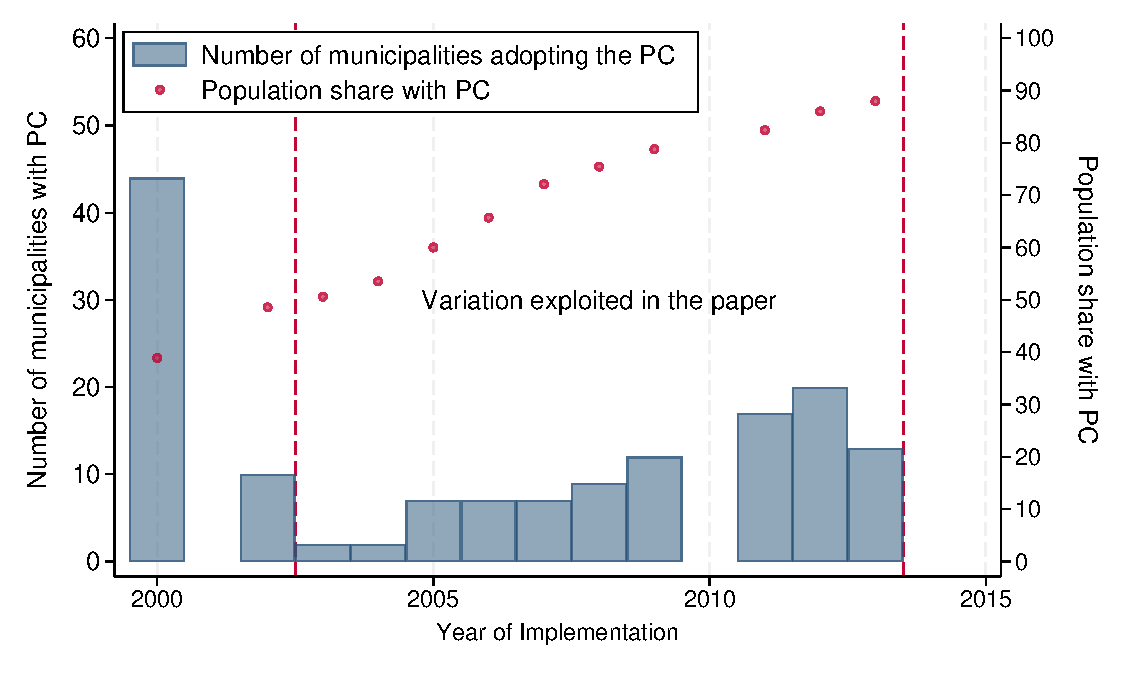
\includegraphics[width=1\textwidth]{../manuscript/Graphs/Graph_PCvariation.pdf}
        \caption{Adoption of \emph{Plan Cuadrante}}
    \end{subfigure}
    \\
    \begin{subfigure}{\textwidth}
    \centering
    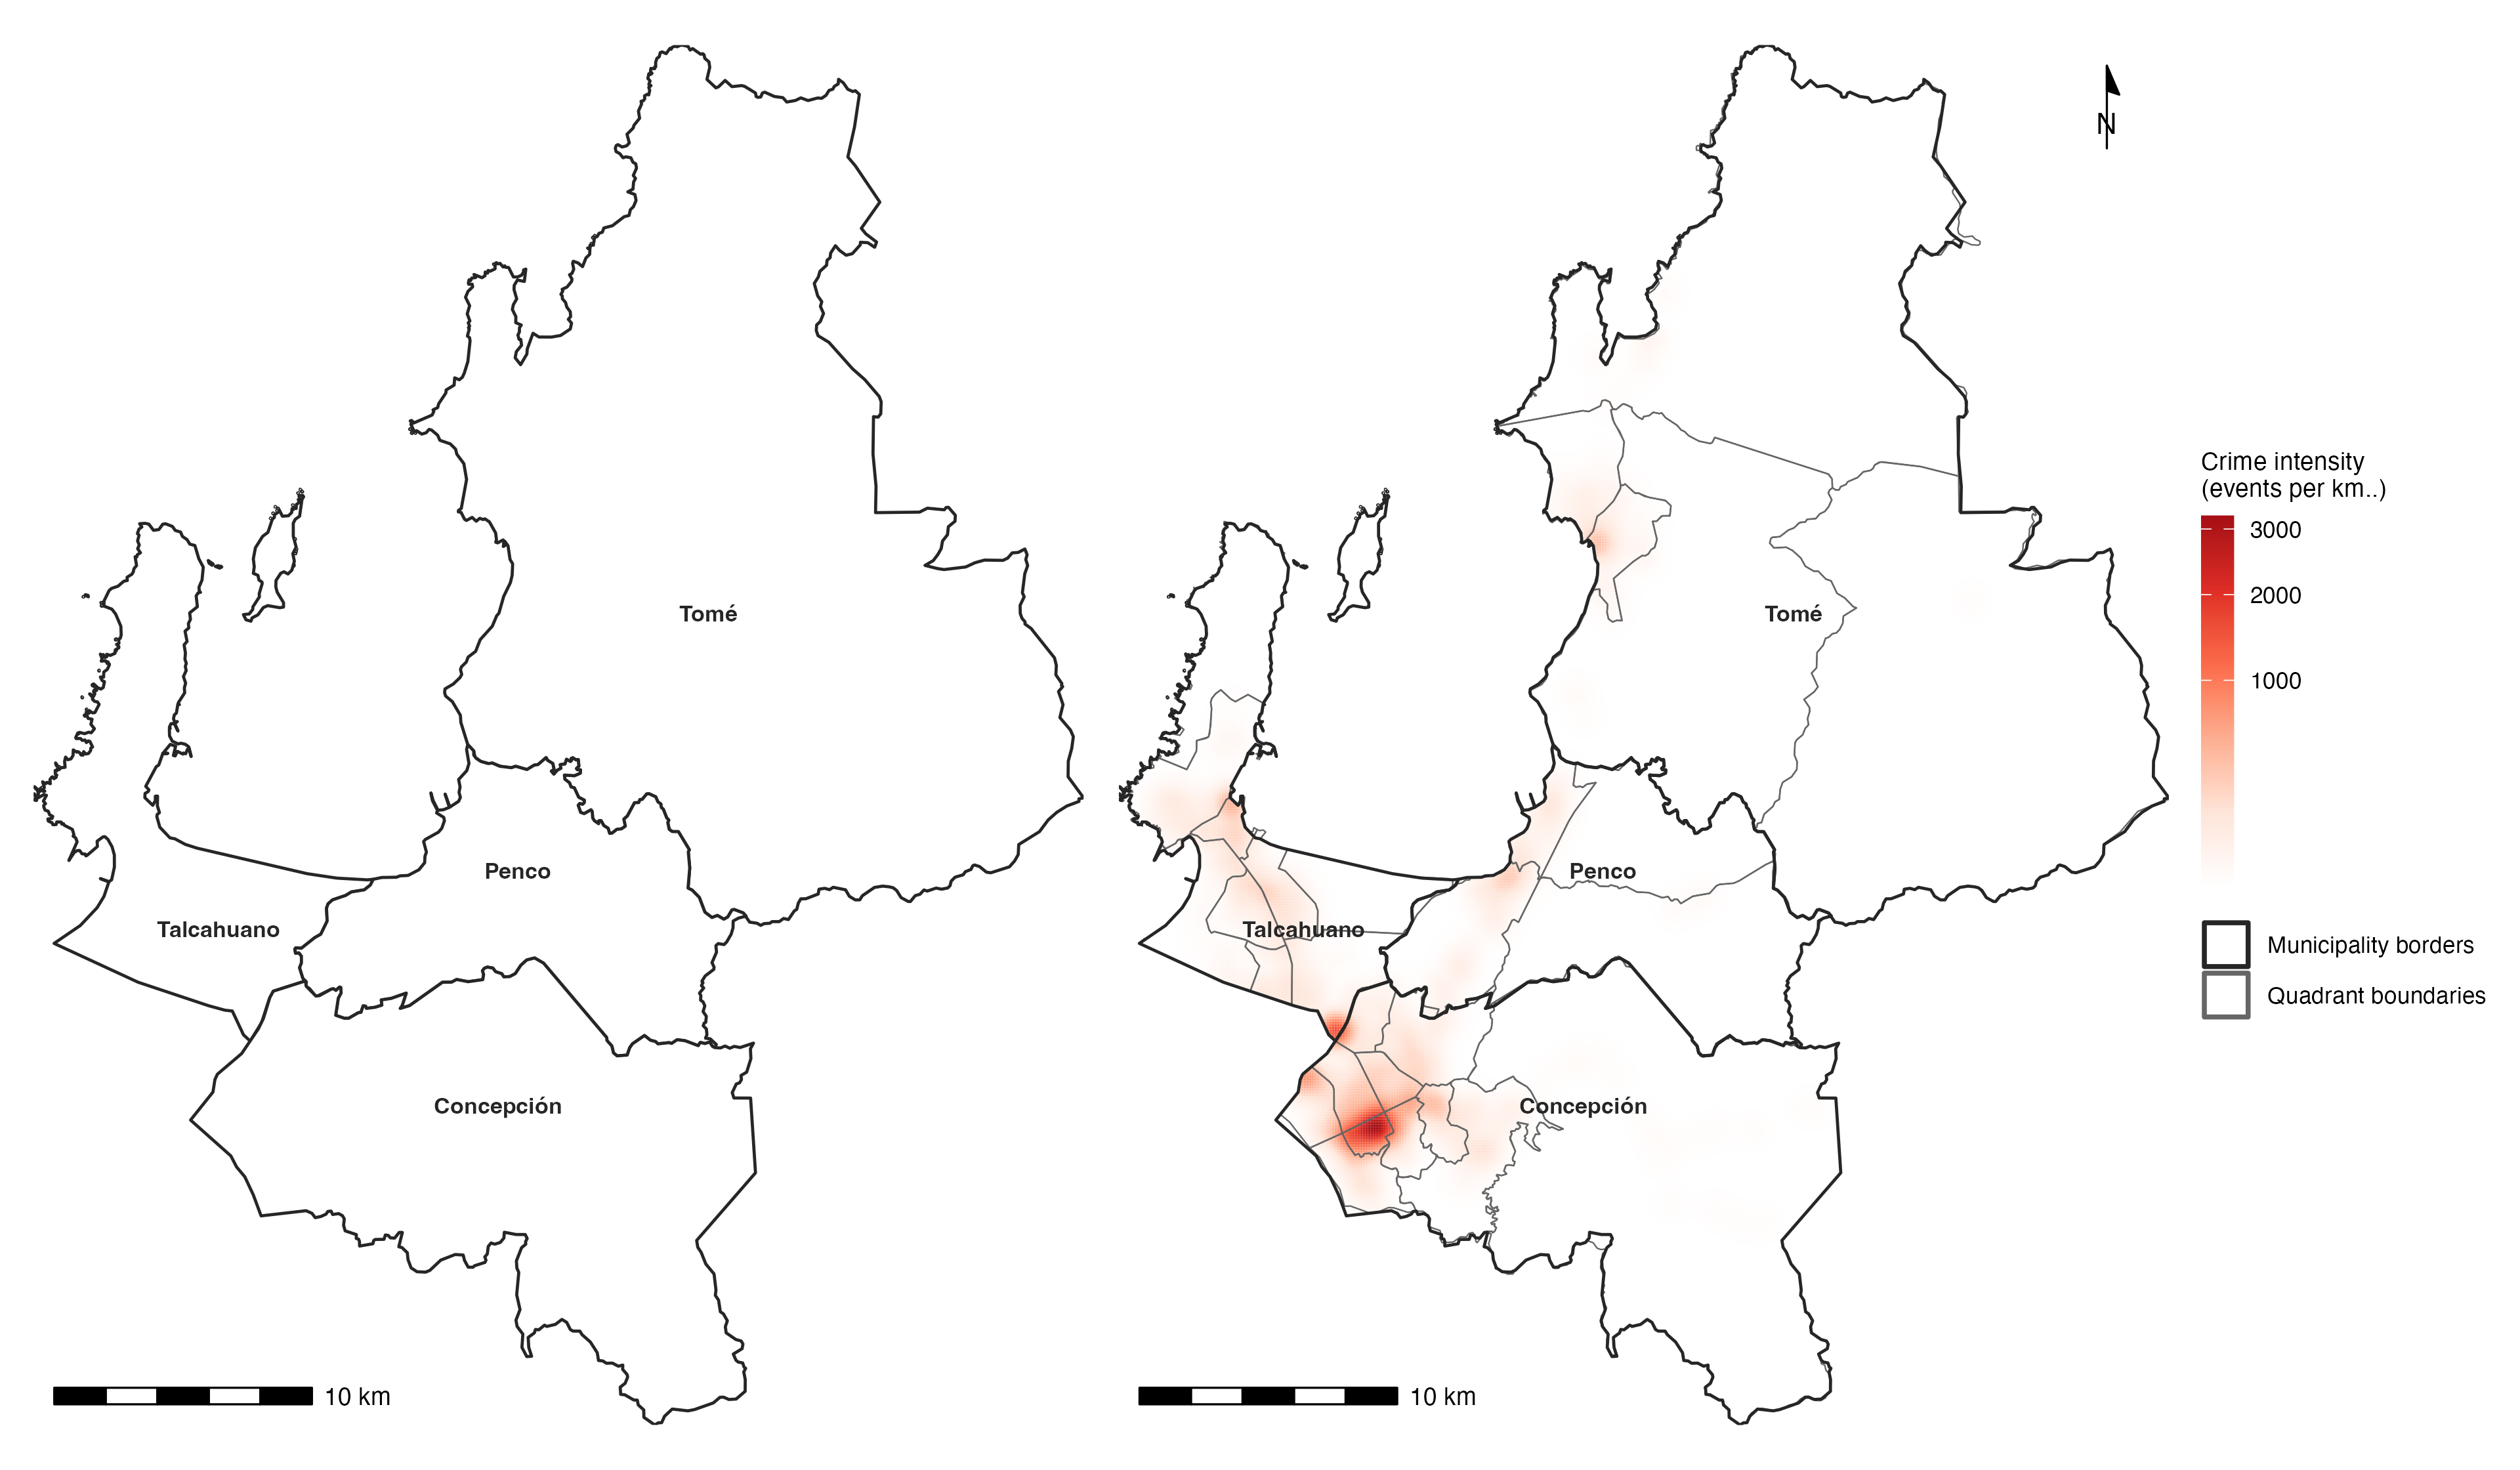
\includegraphics[width=0.65\linewidth]{../manuscript/Graphs/Graph_PCexample_combined.png}
    \caption{\emph{Plan Cuadrante} in the Concepci\'on area}
    \end{subfigure}%
 %   \\
 %   \begin{subfigure}{0.58\textwidth}
 %       \centering
 %       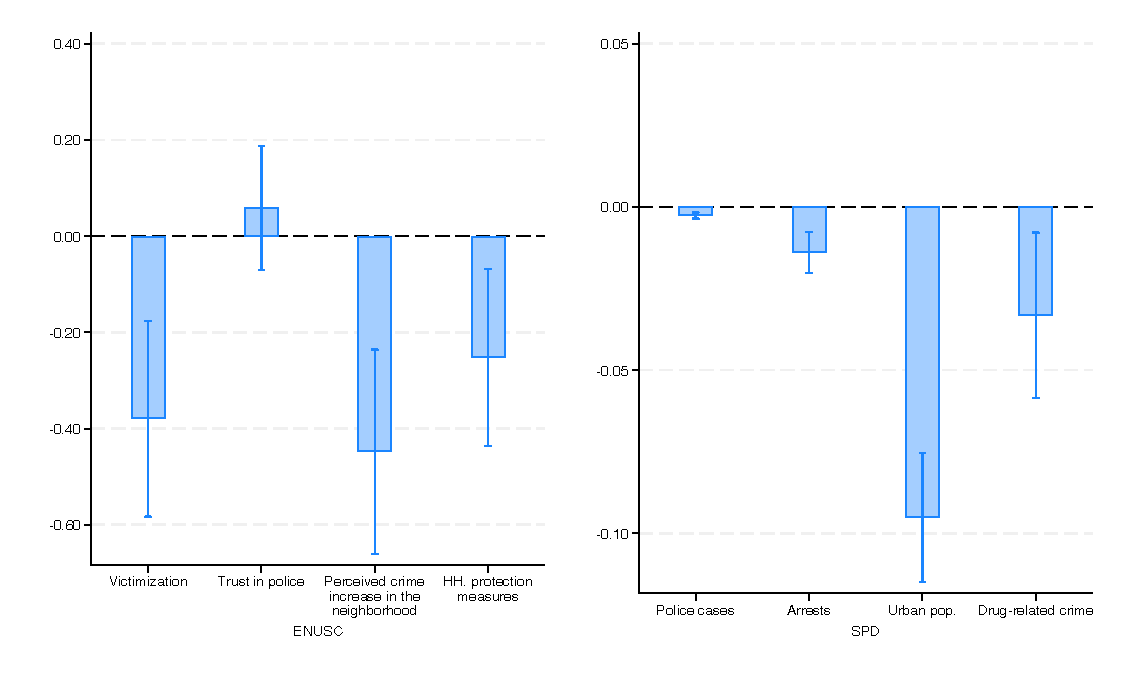
\includegraphics[width=1.1\textwidth]{../manuscript/Graphs/results_predictorsPC_combined.pdf}
 %       \caption{Time of Adoption and Municipality Characteristics}
  %  \end{subfigure}%
    \\[12pt]
    \begin{minipage}{0.95\textwidth}
    \footnotesize Notes: Panel (a) shows the number of municipalities adopting the \emph{Plan Cuadrante} each year (bars), while the circles above them illustrate the cumulative share of the Chilean population living in a municipality with the \emph{Plan Cuadrante} already in place. Panel (b) depicts the metropolitan area of Concepci\'on, the second-largest in Chile: the left map shows its four municipalities---the original police catchment areas---and the right map overlays the Carabineros quadrants together with a kernel-density estimate of all types of robberies and thefts recorded by the police (both reported crimes and arrests). It illustrates how \emph{Plan Cuadrante} subdivided each catchment area (which corresponds to the territory of a municipality) into smaller quadrants, as well as the spatial concentration of crime within them.
    \end{minipage}
\end{figure}
\clearpage

\FloatBarrier

Conceptually, police effectiveness can be viewed as a function of three inputs: total resources, territorial deployment, and policing strategy. Although in some municipalities police resources were increased significantly to operationalize the beat policing model \citep{DIPRES2007_largo,DIPRES2014}, the program primarily transformed the latter two elements. The creation of quadrants was accompanied by permanent geographic assignment of officers to specific areas. This change was operationally critical. By making officers responsible for their quadrant, it encouraged accumulation of local knowledge and stronger community ties, allowing them to adapt patrols and prevention activities to local crime patterns. Importantly, this was not driven by program-specific operational directive changes. Throughout the period we study, a single national set of operational guidelines applied to officers in both treated and control municipalities \citep{Manual_Carabineros2018,DIPRES2007_largo}. Thus, while the average effects we document on crime and crime perception likely reflect combined changes in the three elements we discuss---i.e., resources, deployment, and strategy---the deployment change itself was essential to operationalizing the reform. We discuss the drivers of the effects we document in Section \ref{mechanisms}.

Quadrant size and shape were determined by local police authorities based on factors such as road networks, geographic features, and available resources. In principle, resource allocation across quadrants followed demand for police services, measured in Equivalent Surveillance Units (UVEs); in practice, the station commander retained discretionary authority, as was also the case prior to \emph{Plan Cuadrante} \citep{DIPRES2014}. Municipalities implementing \emph{Plan Cuadrante} were subdivided into an average of seven quadrants, each typically staffed by approximately three officers per shift. On average, each quadrant covered 185 square kilometers and served 13,466 inhabitants. Panel (b) of Figure \ref{fig:figure01} illustrates this structure, showing the 29 quadrants created across the four municipalities of the Concepción metropolitan region---Chile's second-largest metropolitan area and the largest in our sample. Quadrants represented approximately 14\% of the original \emph{comisar\'ia} territory. Officers continued to operate from the same police station but were permanently assigned to a specific sub-area within its jurisdiction. While Carabineros' hierarchical structure limits frontline officer decision-making authority, each quadrant was assigned a Quadrant Delegate (\textit{Delegado de Cuadrante}), a non-commissioned officer, responsible for immediate operational decisions within the quadrant.

\emph{Plan Cuadrante} may affect public safety through two complementary channels: deterrence and police effectiveness, understood as the capacity to respond to and resolve crimes. The changes induced by \emph{Plan Cuadrante}---permanently assigning officers to well-defined neighborhoods and, in some municipalities, increasing available resources---can increase both police visibility and local knowledge. As officers repeatedly patrol the same area, they become familiar with its streets, residents, and routines, which can raise the perceived probability of identification and apprehension and reduce the expected returns to crime. At the same time, this deeper knowledge of local territory and communities can improve police response and case resolution once crimes occur. The reform therefore likely affects both dimensions. Consistent with this interpretation, in Section \ref{results} we document declines in victimization and in reported crime---patterns consistent with deterrence---together with increases in arrests, consistent with improved police effectiveness.

Although beat policing shares features with other policing approaches, such as hot-spot policing and community-based policing, which have been widely studied, it has distinctive features that make it worth studying as an independent approach. Hot-spot policing concentrates resources in high-crime areas and does not focus on building local knowledge and community ties. It is typically implemented through targeted interventions at specific locations rather than systematic territorial organization, and the same officers are not necessarily sent repeatedly to the same areas. Evidence on hot-spot policing is mixed, with some studies showing crime reductions in targeted areas but also potential displacement effects \citep{SR_1}. \emph{Plan Cuadrante}, by contrast, subdivided all urban municipalities into quadrants with permanent officer assignment. As Panel (b) of Figure \ref{fig:figure01} illustrates, some quadrants contained crime hot-spots, but many did not. The reform thus addressed entire urban territories rather than specific high-crime areas, potentially mitigating displacement effects associated with hot-spot policing.

Community-based policing emphasizes building relationships with residents and addressing underlying social issues, and typically involves active community participation in defining strategy and priorities---in some cases, even assuming surveillance and prevention responsibilities. While increasing trust in the police and strengthening community ties were among the declared goals of \emph{Plan Cuadrante}, and may have resulted from its territorial reorganization, the community was not formally involved in the provision of security.\footnote{The \emph{Plan Cuadrante}'s original design contemplated a formal community integration model (MICC) with a Community Affairs Office (\textit{Oficina de Asuntos Comunitarios}) and a dedicated officer in each police station. However, this model was not implemented during our study period. Independent program evaluations from the Budget Office document that these Community Affairs Offices did not exist and had no dedicated personnel, budget, or structured activities in the period we study \citep{DIPRES2007_largo,DIPRES2014}. The community integration model was piloted in four police stations during 2012--2013, none of which are in our analytical sample. Financing was then discontinued in early 2014 and only restored and expanded after our study period ends.}%
 %Similarly, Operations Offices (\textit{Oficina de Operaciones}) formally assigned crime analysis functions but relied on paper-based entry systems, lacking digital infrastructure, analysts, or centralized data systems throughout the study period \citep{DIPRES2014}. Both the community integration model and crime analysis function were substantively implemented only with \emph{Plan Cuadrante} 2.0 (2015--2017) \citep{Carabineros2018}, outside our study period.}

In recent decades, police departments worldwide have transitioned toward beat policing reforms \citep{NASEM2018,PCSP2014}, yet the effectiveness of this model has not been rigorously assessed. Although the beat policing approach introduced through \emph{Plan Cuadrante} shares features with programs previously studied in the economic literature, its distinctive characteristics---comprehensive territorial reorganization and systematic local officer specialization---make it a valuable case for studying how deployment and policing strategies not yet examined in the economics literature affect crime and crime perception.

}
\end{adjustwidth}

\textbf{Mechanisms:} The revised section on mechanisms discusses the drivers of the effects we document, organized around the framework you suggested. Specifically, we investigate the three channels through which \emph{Plan Cuadrante} may affect public security, namely changes in police resources, territorial deployment, and policing strategy. Please note also that figures including data on police resources have changed slightly, as more detailed information on police vehicles and officers became available after the previous manuscript was submitted. The new section reads as follows:\\

\textbf{4.4 What Is Driving the Effects of \emph{Plan Cuadrante}?}
\\[12pt]
\begin{adjustwidth}{2em}{0em}
{\setcounter{figure}{3}\renewcommand{\thefigure}{\arabic{figure}}
%\textbf{4.4 What Is Driving the Effects of \emph{Plan Cuadrante}?}


To reduce crime and improve security perceptions, police forces need to strengthen both prevention and police effectiveness. Both margins can be shaped by resources, territorial deployment, and policing strategy. This section examines which components of \emph{Plan Cuadrante} are most likely to drive the effects documented in Section \ref{results}. 

The central objective of \emph{Plan Cuadrante} was to introduce a beat policing model by reorganizing deployment. Police operational territories that had typically matched municipal boundaries were subdivided into quadrants, and officers were permanently assigned to these quadrants. During our study period, national operational guidelines remained the same in adopting and non-adopting municipalities. Still, this new deployment likely affected policing strategy at a more operational level, because it allowed officers to adapt patrol routes, schedules, and prevention practices using the local knowledge that the program sought to build.

Although changes in resources were not the core of the reform, implementation contemplated increases in municipalities that lacked the personnel and patrol capacity required to move to this model. During the period we study, Chile was expanding public spending on security, and police resources increased in most municipalities regardless of whether or when they adopted \emph{Plan Cuadrante}. On average, however, municipalities adopting the program experienced larger increases in officers and patrol vehicles, as shown in panels (a) and (b) of Figure \ref{fig:resources}. Since increases in police resources have been shown to reduce crime in some contexts \citep{Evans}, this pattern raises a central question for interpretation, namely whether our estimates reflect resource expansion or the deployment and strategy changes introduced by \emph{Plan Cuadrante}. We address this question through a set of exercises that exploit heterogeneity in resource increases across municipalities and over time.

\FloatBarrier
%--- Implementation
\begin{figure}[H]
    \centering
    \caption{Plan Cuadrante and Changes in Police Resources}
    \label{fig:resources}
    \label{fig:figure_resources}
    \begin{tabular}{cc}
        \begin{minipage}[t]{0.48\textwidth}
            \centering
            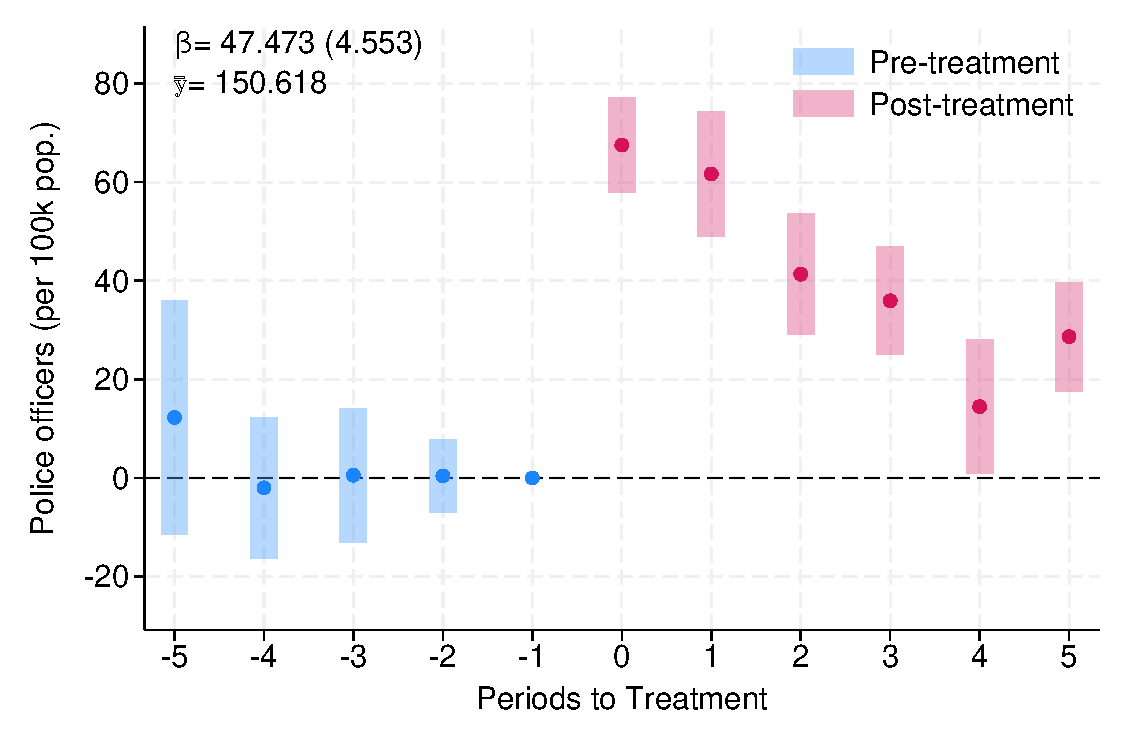
\includegraphics[width=\linewidth]{../manuscript/Graphs/fig4_officers.pdf}

            \small (a) Effect on the number of police officers
        \end{minipage}
        &
        \begin{minipage}[t]{0.48\textwidth}
            \centering
            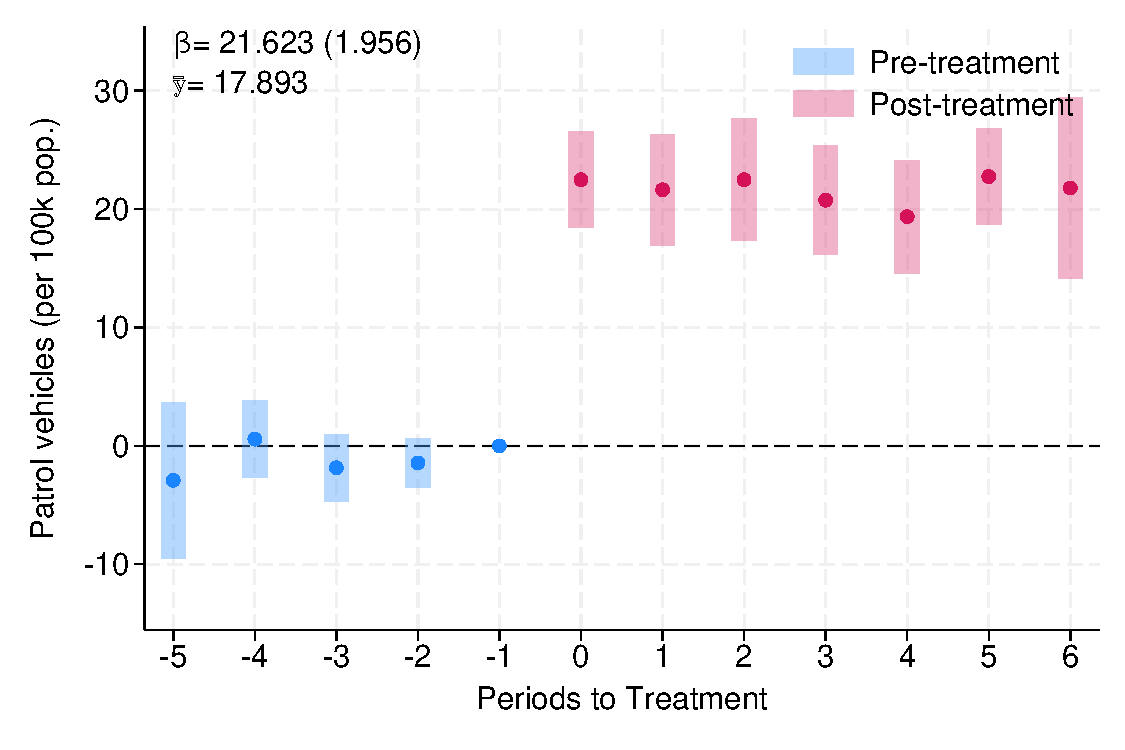
\includegraphics[width=\linewidth]{../manuscript/Graphs/fig4_patrols.pdf}

            \small (b) Effect on the number of patrol vehicles
        \end{minipage}
        \\[4pt]
        \begin{minipage}[t]{0.48\textwidth}
            \centering
            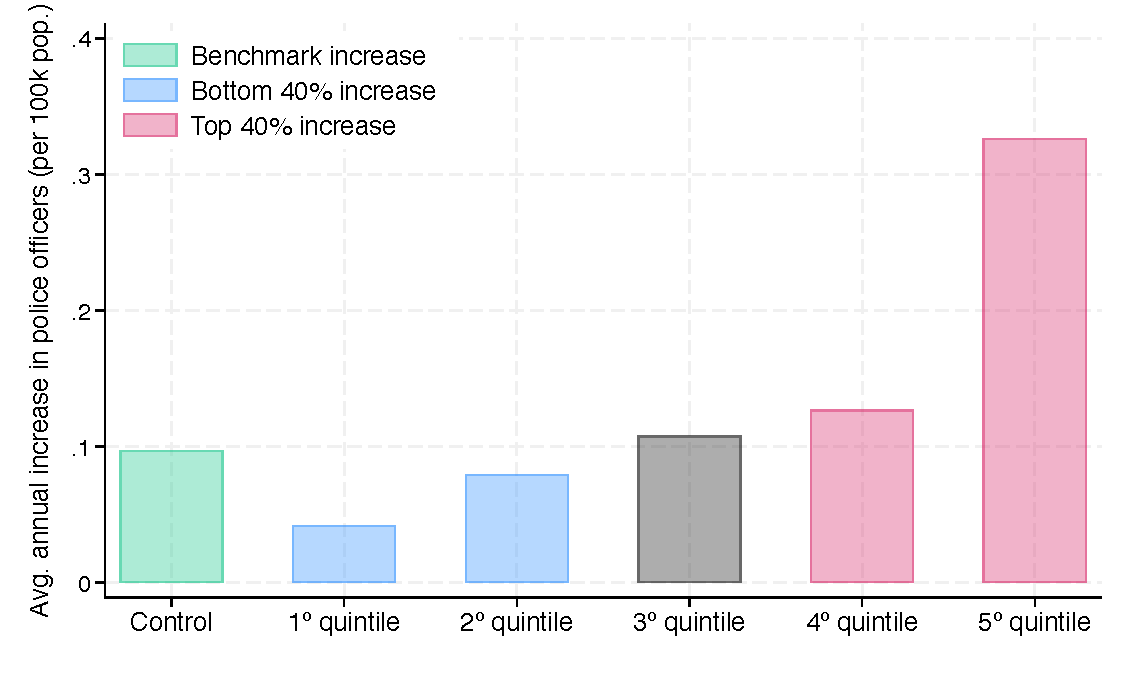
\includegraphics[width=\linewidth]{../manuscript/Graphs/increase_enusc_off_quintiles.pdf}

            \small (c) Distribution of $\Delta$ in police officers
        \end{minipage}
        &
        \begin{minipage}[t]{0.48\textwidth}
            \centering
            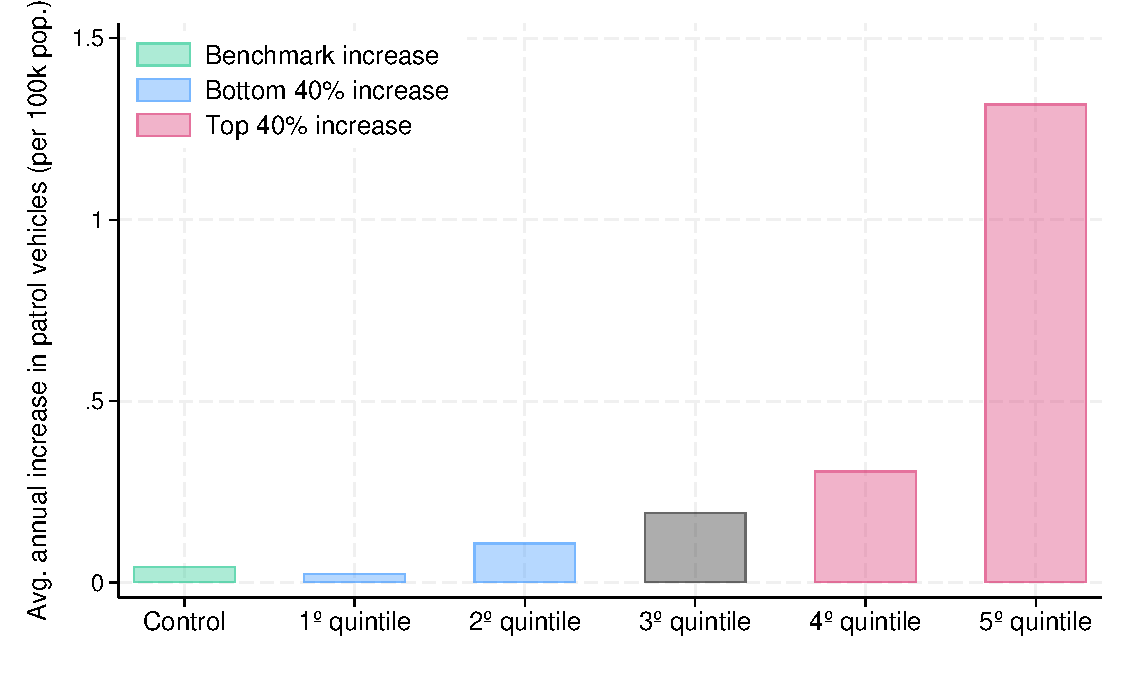
\includegraphics[width=\linewidth]{../manuscript/Graphs/increase_enusc_pv_quintiles.pdf}

            \small (d) Distribution of $\Delta$ in patrol vehicles
        \end{minipage}
        \\[4pt]
        \begin{minipage}[t]{0.48\textwidth}
            \centering
            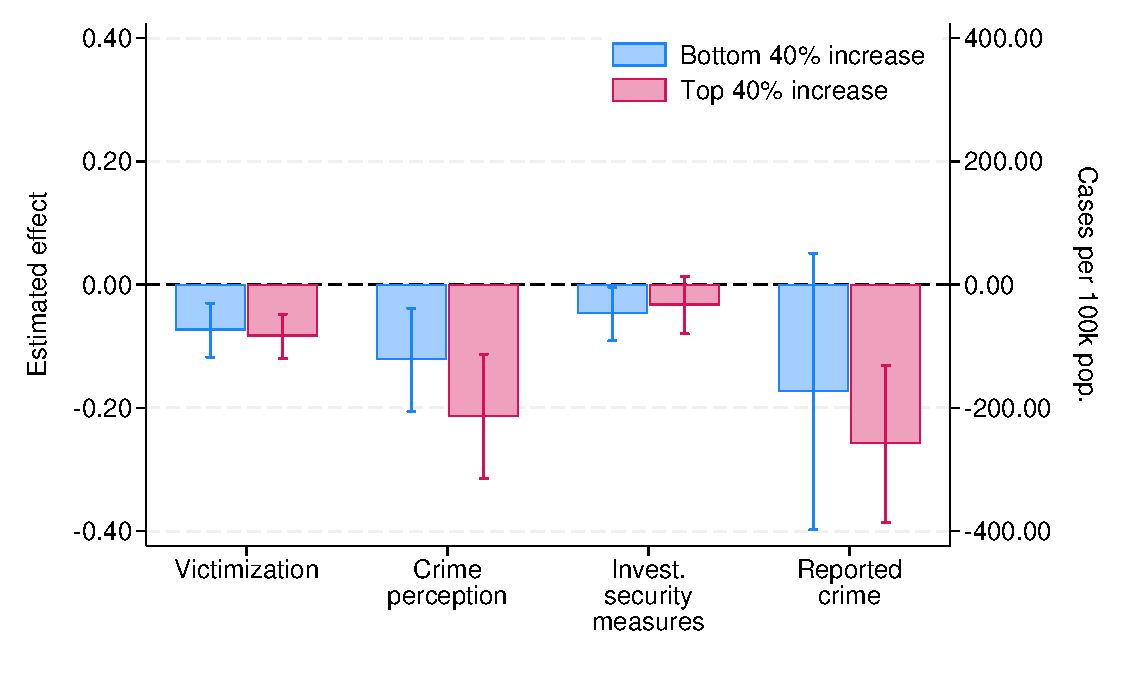
\includegraphics[width=\linewidth]{../manuscript/Graphs/heterogeneity_off.pdf}

            \small (e) Effects by the intensity of $\Delta$ in police officers
        \end{minipage}
        &
        \begin{minipage}[t]{0.48\textwidth}
            \centering
            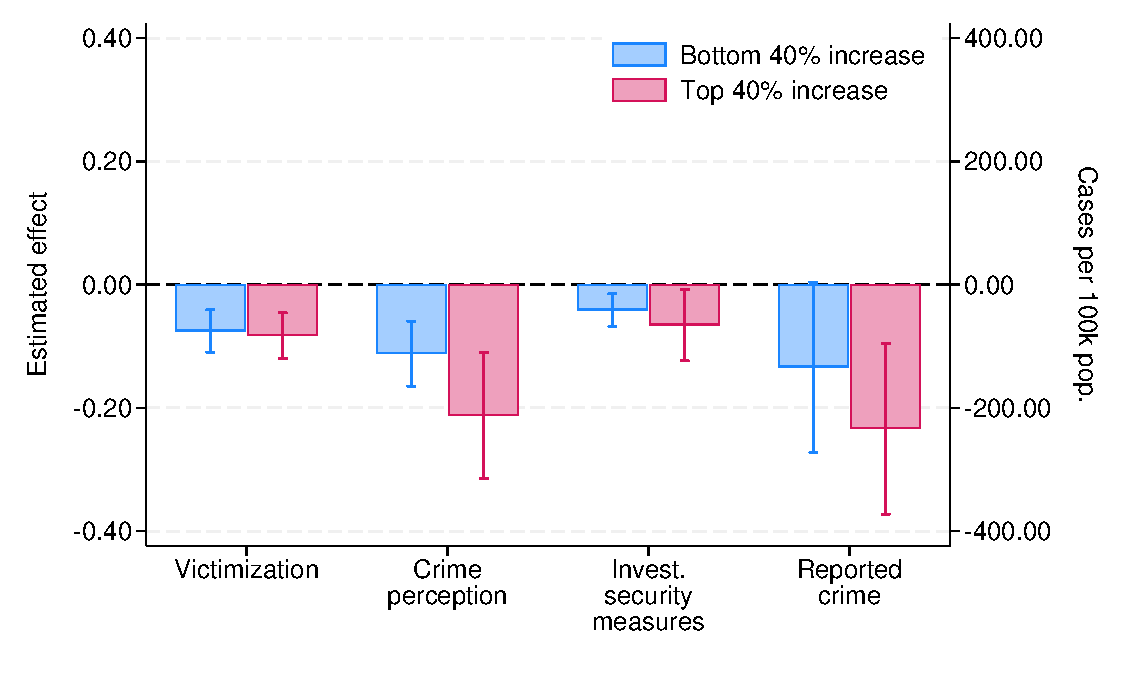
\includegraphics[width=\linewidth]{../manuscript/Graphs/heterogeneity_pv.pdf}

            \small (f) Effects by the intensity of $\Delta$ in patrol vehicles
        \end{minipage}
    \end{tabular}
    \vspace{4pt}
    \begin{minipage}{0.99\textwidth}
    \footnotesize Notes: Panels (a) and (b) show the effect of \emph{Plan Cuadrante} on police officers and patrol vehicles per 100,000 inhabitants. Panels (c) and (d) show the distribution of annual changes in officers and patrol vehicles across municipalities. Panels (e) and (f) report effects by the intensity of resource changes, comparing municipalities in the bottom 40\% and top 40\% of the distribution. The estimation follows \citet{Callaway}. The graphs display estimated coefficients and 95\% confidence intervals. Standard errors are clustered at the municipality level using wild bootstrapping.
    \end{minipage}
\end{figure}
\FloatBarrier
Panels (c) and (d) of Figure \ref{fig:resources} show that the average increase in police resources masks substantial heterogeneity. Municipalities in the bottom 40\% of the resource-change distribution (blue bars) experienced increases close to the average annual variation observed among never treated and not-yet-treated municipalities (green bar). By contrast, municipalities in the top 40\% (red bars) experienced much larger increases, with officers rising by around 22\% and patrol vehicles by around 80\%. If the effects of \emph{Plan Cuadrante} were driven by resource increases alone, we would not expect effects in municipalities whose resource increases were similar to those of the control group. Yet panels (e) and (f) of Figure \ref{fig:resources} show sizeable effects for most crime and crime-perception outcomes even in that low-increase group. While there may be a resource gradient for some crime-perception outcomes, the effects on twelve-month victimization and private investment in security among municipalities with control-like resource increases are close in magnitude to those in municipalities with larger increases. Reassuringly, municipalities in the top and bottom 40\% of the resource-increase distribution do not display differential pre-treatment trends in outcomes or police resources, which suggests that this heterogeneity is not driven by differential pre-existing trends.\footnote{We test for the joint significance of the pre-treatment coefficients between the two groups, separately for the split based on the increase in police officers and the split based on the increase in patrol vehicles. The resulting p-values are, respectively, 0.823 and 0.048 for victimization, 0.059 and 0.379 for crime perception, 0.820 and 0.157 for investment in security measures, and 0.213 and 0.419 for reported crime, as well as 0.616 and 0.444 for police officers and 0.405 and 0.157 for patrol vehicles.}

Although we cannot fully separate the beat policing component from the resource component of the reform---resources may have been important to enable effective implementation of the program, or may explain part of the effects in some municipalities---the fact that municipalities with resource increases similar to those experienced by control municipalities still display sizeable effects indicates that the effects of \emph{Plan Cuadrante} are not driven entirely by resources.\footnote{We also re-estimate the results in Figure \ref{fig:figure02} but controlling for police resources. Online Appendix Table \ref{tab:results_controlbyresources} shows that the magnitude of the estimated effects remains similar for most variables, although the statistical significance is reduced in some estimations. This likely reflects a mechanical feature of the \citet{Callaway} estimation procedure: control variables are not incorporated parametrically, but are instead used to construct the comparison group via outcome regression or propensity-score weighting, so the resulting estimation uncertainty propagates to the ATT standard errors. Note, in addition, that police resources are a bad control---i.e., at least part of their variation is a result of the adoption of \emph{Plan Cuadrante}---so these results should be interpreted cautiously.}\footnote{Table \ref{tab:resourcecorrelates} in Online Appendix \ref{sec:appendixB} examines which factors are associated with a larger increase in police resources upon the adoption of \emph{Plan Cuadrante}.}


\FloatBarrier
%--- Implementation
\begin{figure}[h!]
    \centering
    \caption{Police Resources and Public Safety}
    \label{fig:resources2}
    \begin{subfigure}[t]{0.55\textwidth}
        \centering
        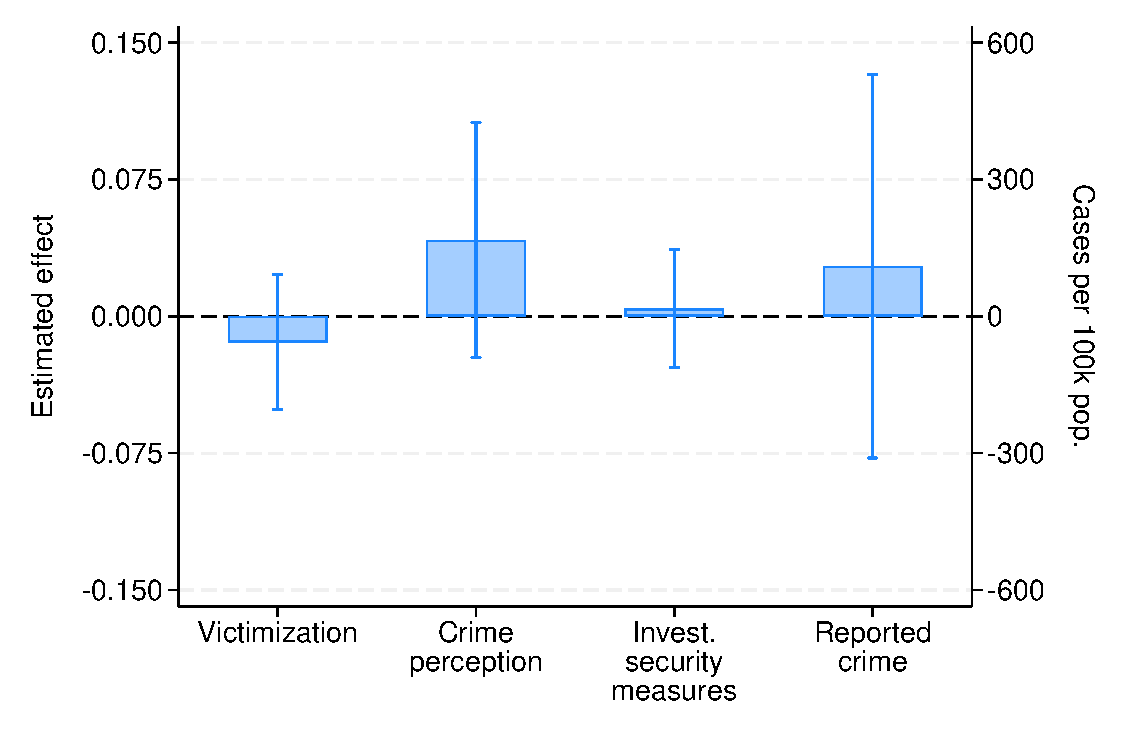
\includegraphics[width=\linewidth]{../manuscript/Graphs/results_SC_att_combined.pdf}
        \caption{Effects of \emph{Seguridad Ciudadana}}
    \end{subfigure}
    \\[6pt]
    \begin{subfigure}[t]{0.55\textwidth}
        \centering
        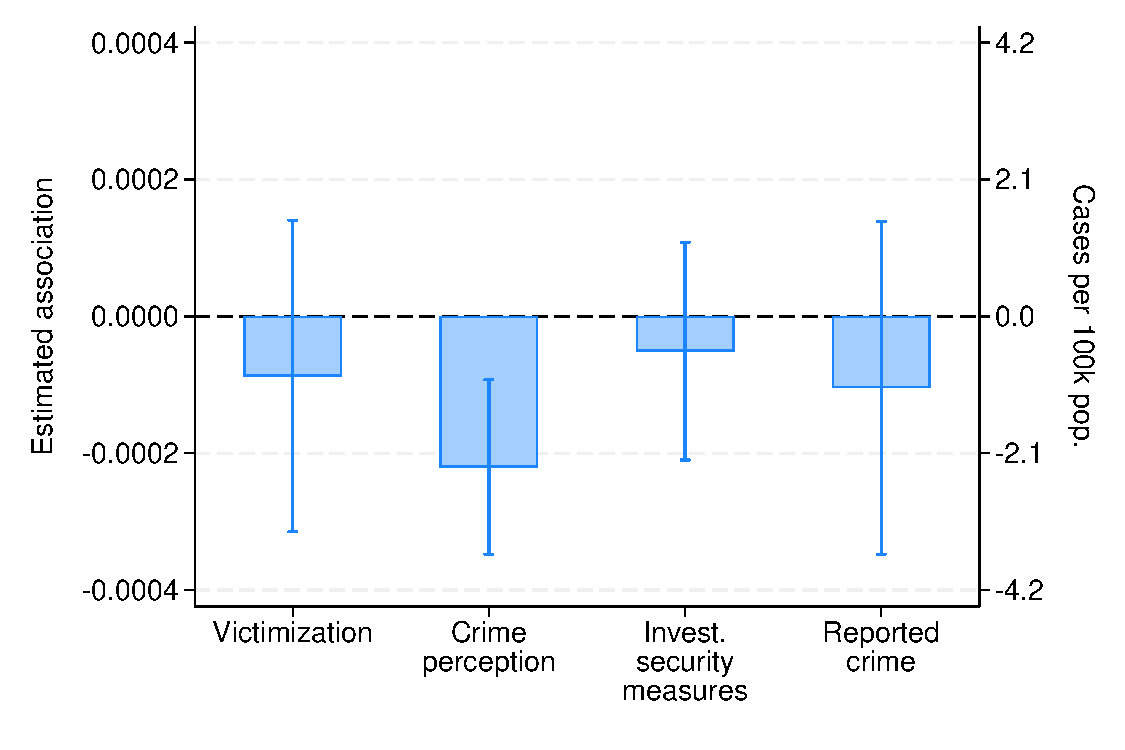
\includegraphics[width=\linewidth]{../manuscript/Graphs/results_corr_novariation_off_santiago.pdf}
        \caption{Association between police officers and effectiveness}
    \end{subfigure}
    \\[6pt]
    \begin{subfigure}[t]{0.55\textwidth}
        \centering
        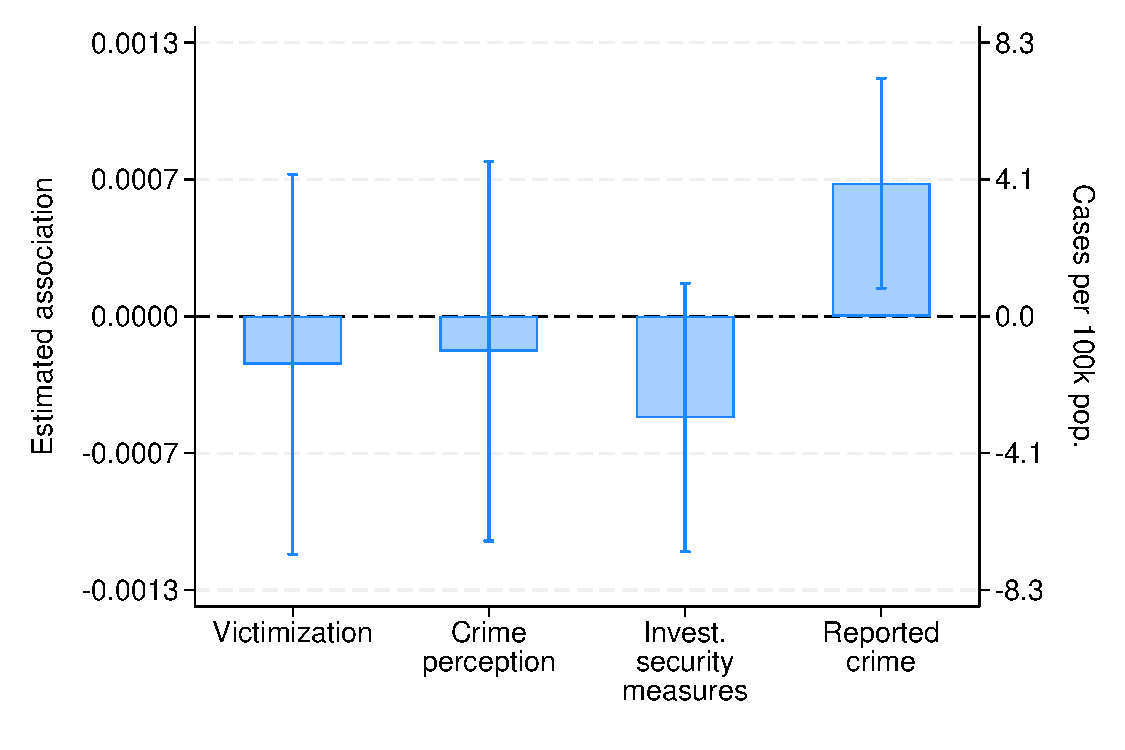
\includegraphics[width=\linewidth]{../manuscript/Graphs/results_corr_novariation_veh_santiago.pdf}
        \caption{Association between patrol vehicles and effectiveness}
    \end{subfigure}
    \\[8pt]
    \begin{minipage}{0.99\textwidth}
    \footnotesize Notes: Panel (a) reports the pooled effect of \emph{Seguridad Ciudadana}, a program that expanded local security personnel to support patrolling and deterrence but did not replicate the deployment-and-strategy features of \emph{Plan Cuadrante}. Panels (b) and (c) report within-municipality associations between police resources and police-effectiveness outcomes among the 41 municipalities of the Santiago Metropolitan Region, all of which had adopted \emph{Plan Cuadrante} by 2000. The regressions include municipality and year fixed effects. Standard errors are clustered at the municipality level using the wild bootstrapping procedure.
    \end{minipage}
\end{figure}
\FloatBarrier

To further investigate whether resource increases alone can explain our results, we assess the effects of \emph{Seguridad Ciudadana}, a program that expanded local security personnel to support patrolling and deterrence, but did not replicate the core deployment-and-strategy features of \emph{Plan Cuadrante}. Using a difference-in-differences specification following \citet{Callaway}, panel (a) of Figure \ref{fig:resources2} shows no significant effects of these resource changes on police effectiveness. Further details about this exercise and the corresponding event-study estimates are reported in Online Appendix \ref{sec:appendixB} and Online Appendix Figure \ref{fig:figureA5}. 


Finally, we study whether variation in police resources in municipalities that had already adopted \emph{Plan Cuadrante} improves public safety and security perceptions. Using ENUSC data and information on resources for 2006--2012 in the 41 municipalities of the Santiago Metropolitan Region---all of which had adopted \emph{Plan Cuadrante} by 2000---we exploit variation in officers and patrol vehicles that is unrelated to program adoption. Panels (b) and (c) of Figure \ref{fig:resources2} show the association between police resources and our main outcomes, conditional on municipality and year fixed effects. With one exception---the association between police officers and crime perception---none of these associations is statistically significant at conventional confidence levels. \footnote{Online Appendix Figure \ref{fig:figureA7B} reports the same exercise and also shows similar results for the broader set of municipalities that adopted \emph{Plan Cuadrante} before 2006 and never-treated municipalities (red bars); see Online Appendix \ref{sec:appendixB} for further details.}

Taken together, these results suggest that resource increases alone do not account for the effects of \emph{Plan Cuadrante}. We next turn to evidence that speaks more directly to the beat-policing components of the reform.

Panel (a) of Figure \ref{fig:police_performance} shows that, following the adoption of \emph{Plan Cuadrante}, households are much more likely to report increased police presence in their neighborhoods. The share of households perceiving increased police presence rises by 35 percentage points (156\%), the share reporting that police pass by their house daily rises by 22 percentage points (59\%), the share reporting never seeing police patrols near their house falls by 10 percentage points (57\%), and complaints about lack of police surveillance fall by around 5 percentage points (20\%). This evidence is consistent with both larger resources and the new deployment model. Yet the latter estimate---the only police-presence outcome for which we can separately estimate effects in municipalities with small and large resource increases---is similar in magnitude across the two groups, which suggests that the increase in police presence is not explained only by larger resource increases (see Online Appendix Figure \ref{fig:heterogeneity_appendix}).\footnote{We cannot estimate heterogeneous effects for other police-presence outcomes, such as the reporting of police passing by or the share of households perceiving an increase in police presence, because those variables are available only in ENUSC rounds 2003, 2005, and 2006, while resource data start in 2006.} More importantly, the broader pattern of results suggests that \emph{Plan Cuadrante} did more than simply increase patrolling intensity. Existing work shows that police presence can reduce crime while officers are present, but that its overall effects may be attenuated when crime is displaced across places or time windows \citep{MASTROBUONI2019, Blanes_Mastrobuoni_2018}. Our results point to something broader. As discussed in Section \ref{results}, we find actual declines in victimization and reported crime, together with no evidence of spillovers to neighboring municipalities. This pattern is more consistent with officers accumulating local knowledge and adapting prevention strategies to local conditions under stable territorial assignment than with a purely mechanical increase in patrol intensity.

Panel (b) of Figure \ref{fig:police_performance} reinforces this interpretation. Households in early-adopting municipalities report better police performance across multiple dimensions. They are 8.1 percentage points (16\%) more likely to rate police performance as good or very good, 7.6 percentage points (11\%) more likely to describe police as efficient, 5 percentage points (6\%) more likely to report that police are helpful, and 4.9 percentage points (7\%) more likely to report that police are well informed. They are also 3.9 percentage points (10\%) less likely to perceive police as corrupt, 7.9 percentage points (21\%) less likely to believe police fail to control crime, and 7.6 percentage points (22\%) less likely to report that police do not perform their duties effectively.\footnote{Information on police performance is only available in ENUSC round 2005. Using this round, we compare perceived police performance in municipalities that adopted \emph{Plan Cuadrante} in 2005 or earlier and in municipalities adopting after 2005. Figure \ref{fig:balance_doseresponse} in Online Appendix \ref{sec:appendixB} shows that the number of years of exposure to \emph{Plan Cuadrante} is positively correlated with perceived police performance. While these exercises on perceived police performance should be interpreted with caution, we show in the same appendix that the timing of future adoption is not correlated with perceived police performance in 2005 for municipalities that had not yet adopted the program by 2005.} %These perceived improvements are consistent with a setting in which officers become better informed about local routines and more effective in how they patrol and respond.

The administrative evidence points in the same direction. Panel (c) of Figure \ref{fig:police_performance} shows that arrests per 100,000 inhabitants increase by 48 (14\%) in our main estimates, even as crime declines overall.\footnote{As with reported crime, this event study is restricted to 5 pre-treatment and 7 post-treatment periods for symmetry with the ENUSC-based analysis; Online Appendix Figure \ref{fig:admin_uncapped} reports the results for arrests using the full set of pre-treatment and post-treatment periods.} This effect is also significant among municipalities with resource increases similar to those in the control group (see Online Appendix Figure \ref{fig:heterogeneity_appendix}). Consistent with this pattern, panel (d) of Figure \ref{fig:police_performance} shows that the arrest rate per reported crime also increases by 1.7 percentage points (10\%), suggesting that a higher share of crimes reported to the police are being solved. Because these gains appear even where resources did not increase more than in control municipalities, they are difficult to reconcile with a pure resource story and are more naturally interpreted as improvements in police effectiveness under the deployment and strategy changes introduced by \emph{Plan Cuadrante}. The corresponding event-study estimates for arrests, the arrest rate per reported crime, and trust in the police in Figure \ref{fig:police_performance} confirm that these changes emerge only after adoption.

Finally, panel (e) of Figure \ref{fig:police_performance} shows a sharp increase in trust in the police in our main specification (Section \ref{results}), consistent with one of the objectives of beat policing, namely bringing officers closer to the community and allowing them to accumulate local knowledge through repeated interaction. Online Appendix Figure \ref{fig:heterogeneity_appendix} shows that this effect remains sizeable both in municipalities that experienced resource increases similar to the control group and in those with larger increases.

Overall, although resources were likely important for implementation and may explain part of the effects in some municipalities, the results in this section indicate that resource changes alone are not enough to explain our findings. The evidence is more consistent with a combination of deployment changes and the strategy adjustments enabled by local knowledge accumulation under permanent assignment to quadrants.

\FloatBarrier
%--- Implementation
\begin{figure}[!ht]
    \centering
    \caption[\emph{Plan Cuadrante} and Changes in Police Performance]{\emph{Plan Cuadrante} and Changes in Police Performance}
    \label{fig:figure05}
    \label{fig:police_performance}
    \label{fig:effectiveness_es}
    \begin{subfigure}[t]{0.44\textwidth}
        \centering
        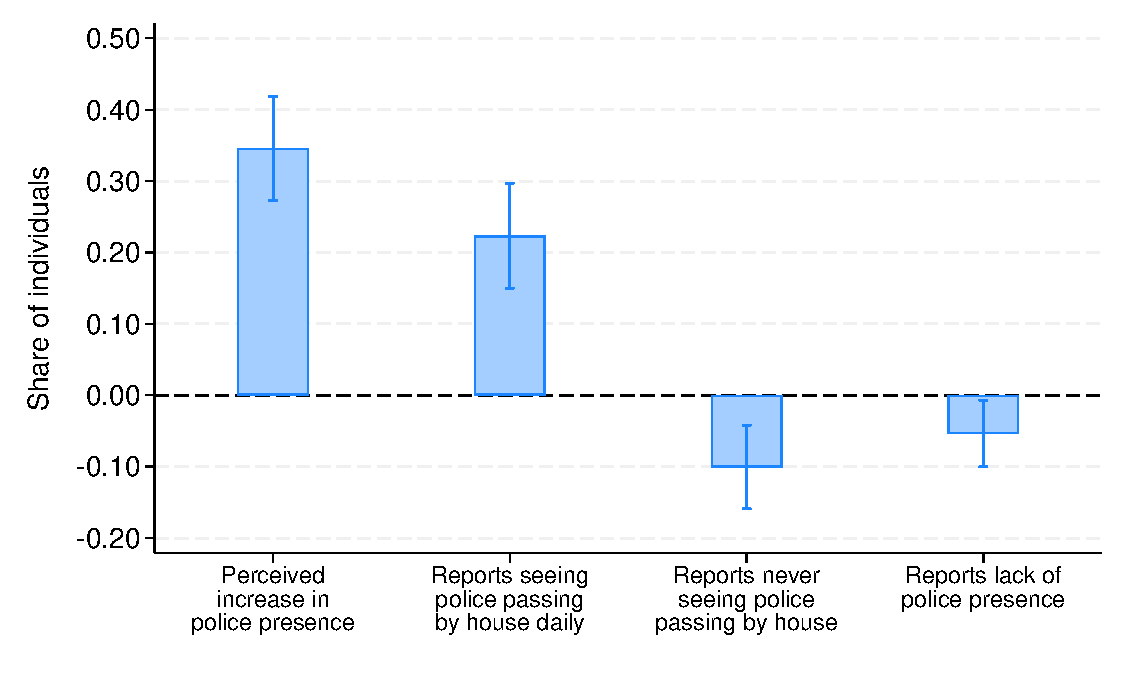
\includegraphics[width=\linewidth]{../manuscript/Graphs/results_policepresence.pdf}
        \caption{Effect on police presence}
    \end{subfigure}\hfill
    \begin{subfigure}[t]{0.44\textwidth}
        \centering
        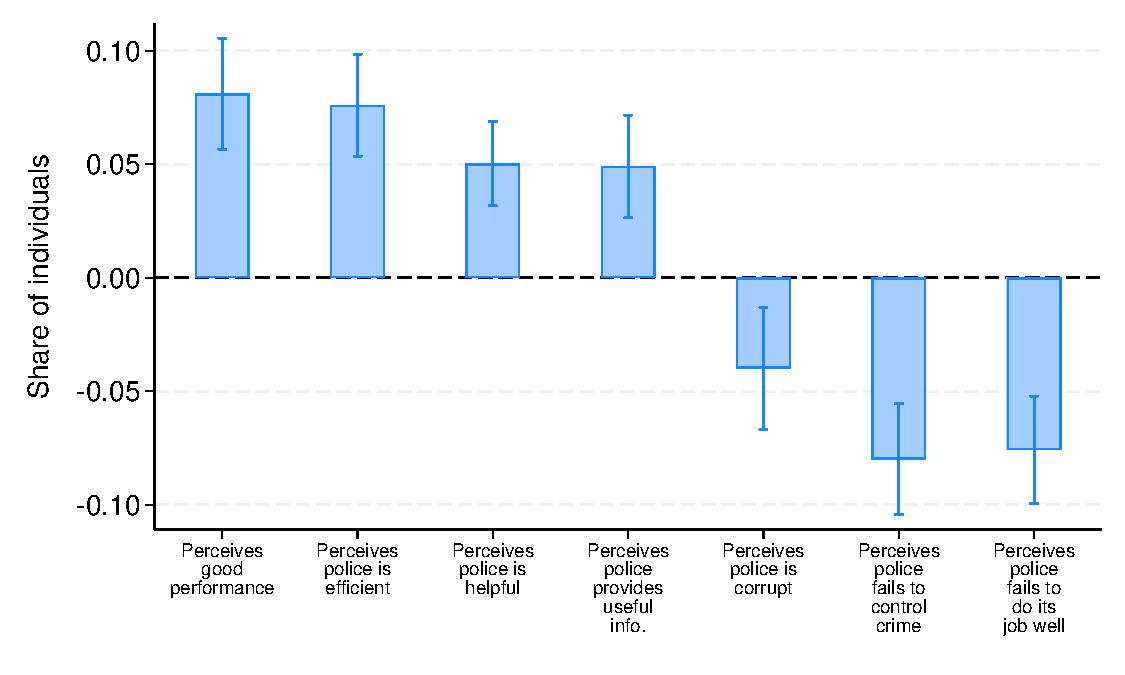
\includegraphics[width=\linewidth]{../manuscript/Graphs/combined_PCttest_2.pdf}
        \caption{Effect on perceived police performance}
    \end{subfigure}
    \\[6pt]
    \begin{subfigure}[t]{0.44\textwidth}
        \centering
        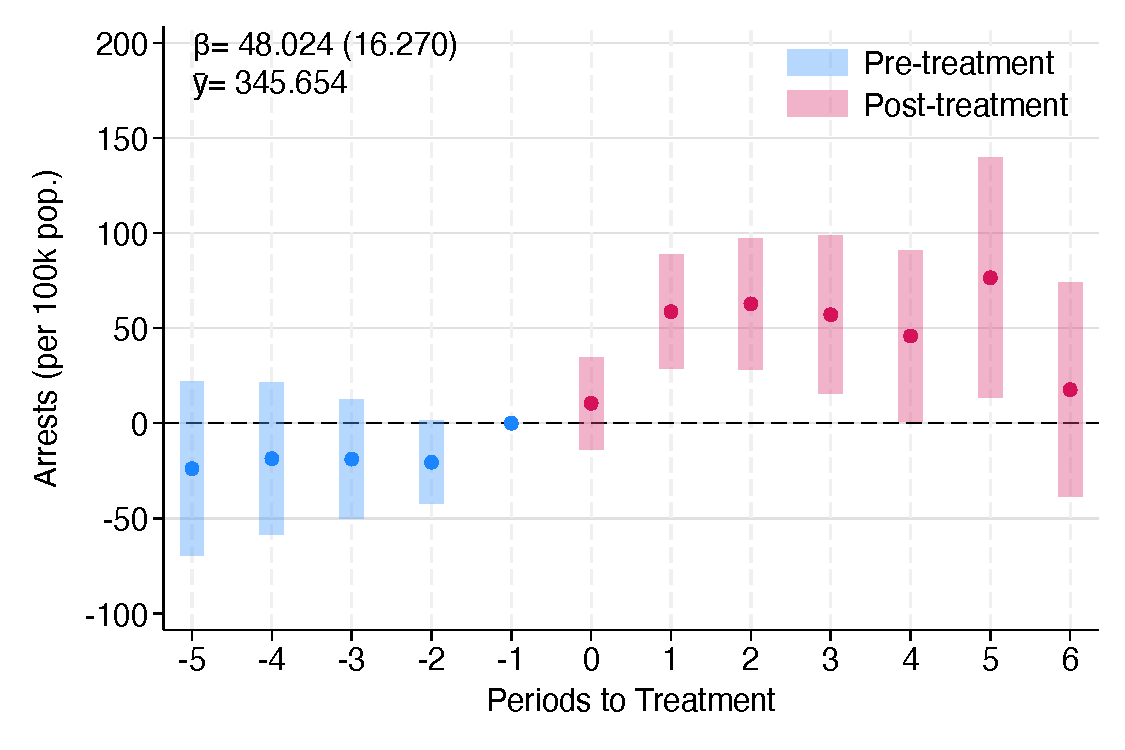
\includegraphics[width=\linewidth]{../manuscript/Graphs/totalarrestscrime_allcomunas.pdf}
        \caption{Arrests (per 100k pop.)}
    \end{subfigure}\hfill
    \begin{subfigure}[t]{0.44\textwidth}
        \centering
        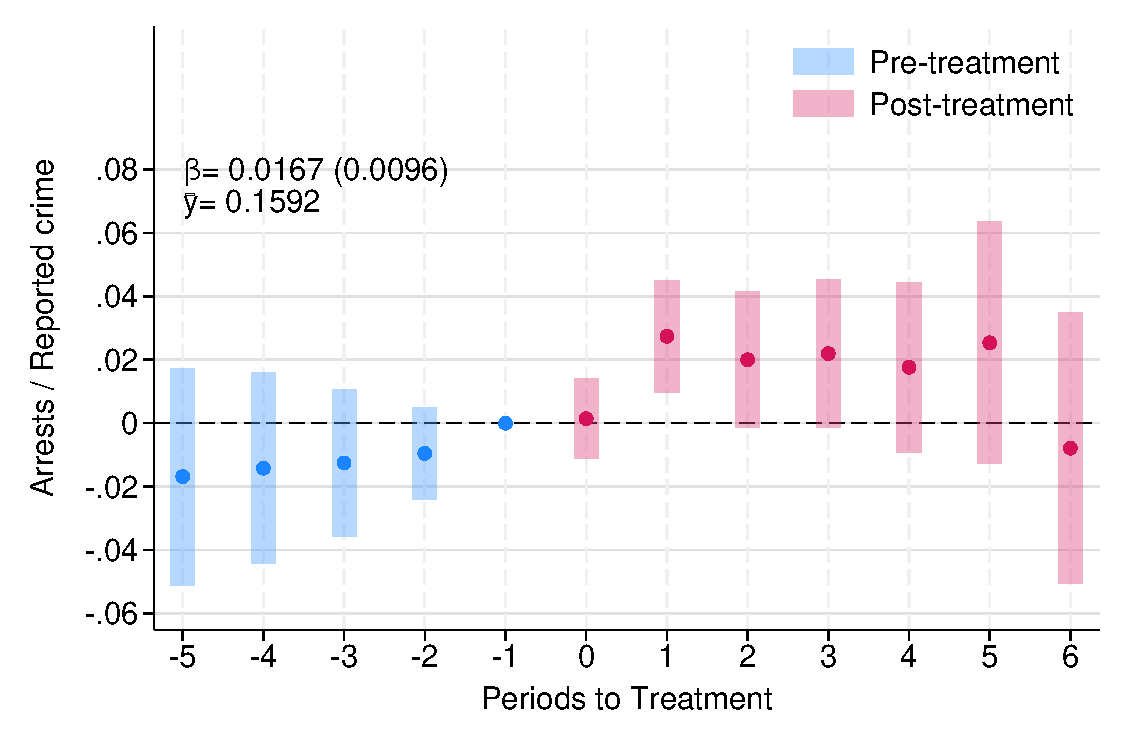
\includegraphics[width=\linewidth]{../manuscript/Graphs/arrests_over_reportedcrime_allcomunas.pdf}
        \caption{Arrests / Reported crime}
    \end{subfigure}
    \\[6pt]
    \begin{subfigure}[t]{0.44\textwidth}
        \centering
        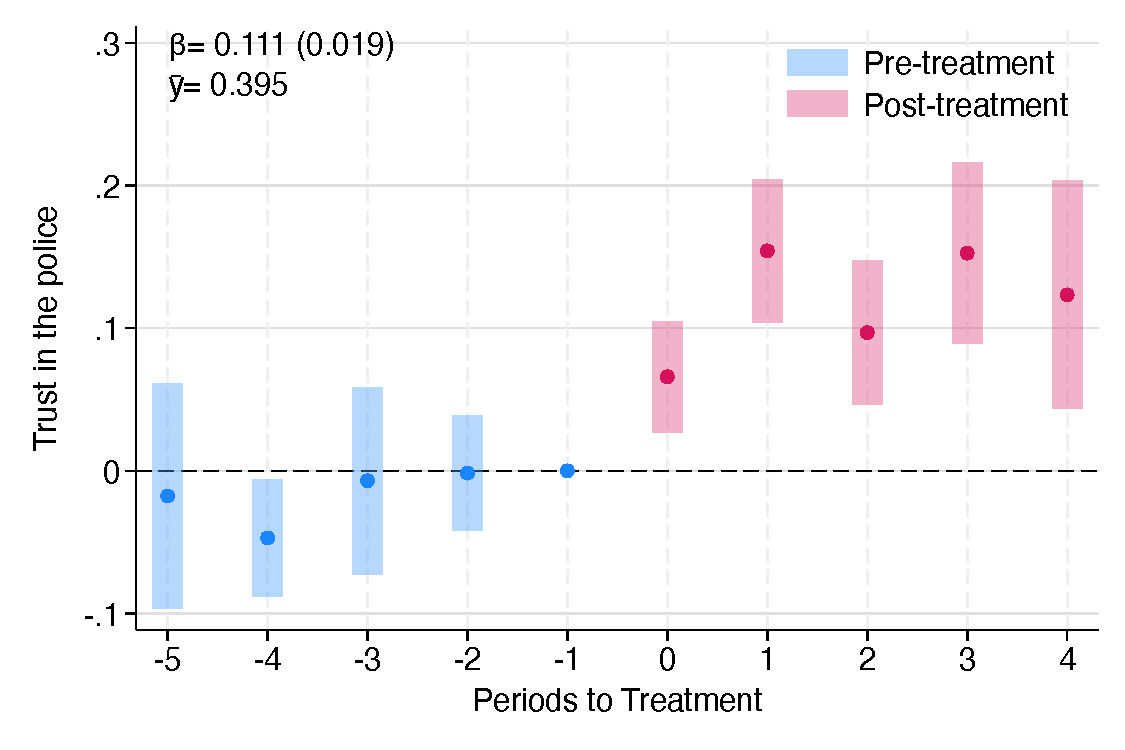
\includegraphics[width=\linewidth]{../manuscript/Graphs/results_trustcarabineros.pdf}
        \caption{Trust in the police}
    \end{subfigure}
    \\[8pt]
    \begin{minipage}{0.99\textwidth}
    \footnotesize Notes: Panel (a) reports the effects on perceived police presence. Panel (b) reports perceived police performance in 2005, comparing municipalities where \emph{Plan Cuadrante} was already implemented before 2006 with municipalities where it was implemented after 2005. Panels (c), (d), and (e) report dynamic event-study estimates for arrests per 100,000 inhabitants, the ratio of arrests to reported crime, and trust in the police. The estimation follows \citet{Callaway}. The graphs display estimated coefficients and 95\% confidence intervals. Standard errors are clustered at the municipality level using the wild bootstrapping procedure.
    \end{minipage}
\end{figure}

\FloatBarrier

%Overall, while resources were arguably important for implementation, the evidence suggests that the beat policing elements---permanent assignment of officers to quadrants and greater local knowledge---were important drivers of the improvements in public safety and security perceptions we document in the paper.



 
}
\end{adjustwidth}

\textbf{Conclusion:} the new conclusion reads as follows:\\
\begin{adjustwidth}{2em}{0em}
Beat policing---i.e., assigning the same officers to smaller, well-defined territorial units rather than rotating them over larger ones---has become a widespread strategy to address crime and maintain public safety, yet rigorous causal evidence on its effectiveness remains scarce. Using administrative and survey data from Chile, we show that \emph{Plan Cuadrante}, a reform that introduced beat policing in urban municipalities, substantially reduced victimization and crime perception, while increasing trust in the police. Although its implementation required increasing police resources in some municipalities, we show that resource increases alone cannot account for the observed improvements. The beat policing elements of the reform---permanent assignment to quadrants enabling officers to build local knowledge---seem to be key drivers of its effectiveness.

The reform not only reduced crime incidence but also insecurity perceptions. As a result, households in adopting municipalities reduced their investment in private security measures. Crime rates and perceived victimization risk do not always move together \citep{Ajzenman_Pato}, yet \emph{Plan Cuadrante} reduced both simultaneously. This is an important result as misalignments between actual and perceived risk can lead households to overinvest in private security and distort public expenditure priorities \citep{Minali, Ajzenman_Pato}.

The reform also increased trust in the police---an outcome that has proven particularly difficult to achieve in low- and middle-income countries. Community policing, long regarded as the primary strategy for building police legitimacy, has shown limited effects on both crime and trust in such settings \citep{blair2021, Tobon}. Beat-policing takes a different approach. Rather than relying on community co-production of security, it builds proximity and trust organically through sustained, stable territorial engagement. Our results suggest this organizational logic can be effective even outside developed-country contexts.

Taken together, these results contribute to a broader body of evidence that highlights that the spatial organization of police resources matters. By assigning officers permanently to smaller territorial units, beat policing increases visibility, deepens local knowledge, and improves the capacity of officers to prevent crime and respond to it effectively. This pattern echoes findings from health and education showing that aligning frontline service providers more closely with the communities they serve enhances outcomes \citep{besley2003centralized, Bardhan, Bloom_2015, Basurto}.

While \emph{Plan Cuadrante} was implemented under specific conditions, those conditions help clarify when beat policing is likely to succeed. Two institutional features appear particularly important. First, the absence of significant organized crime during the study period allowed officers to operate repeatedly in their assigned areas without meaningful risk of intimidation or capture, enabling local knowledge and community ties to take root. Second, the relatively high level of professional training in the Chilean police provided a foundation for effectively implementing the reform. Neither of these features is idiosyncratic. They describe an institutional environment that is present, or could be developed, in many settings. Together, they suggest that the gains from beat policing are most likely to materialize when supported by a capable police force operating in a security environment where persistent local engagement is feasible.
\end{adjustwidth}

\clearpage
\noindent\textbf{Other figures and tables referenced above:}
\vspace{0.5em}

{\setcounter{figure}{1}\renewcommand{\thefigure}{\arabic{figure}}
%--- Implementation
\begin{figure}[h!]
    \centering
    \caption{Effects of \emph{Plan Cuadrante} on Crime Outcomes and Security Perceptions}
    \label{fig:figure02}
    \begin{subfigure}{0.495\textwidth}
        \centering
        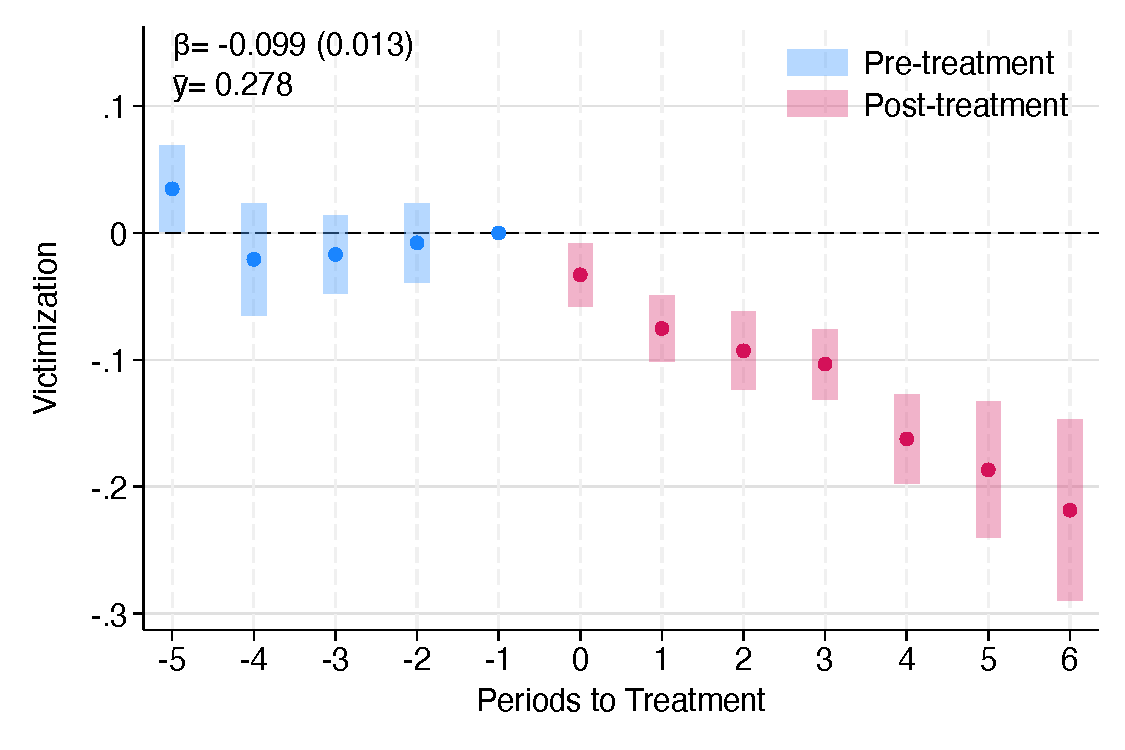
\includegraphics[width=\textwidth]{../manuscript/Graphs/results_victimization.pdf}
        \caption{Victimization in last 12 months}
    \end{subfigure}%
    ~
    \begin{subfigure}{0.495\textwidth}
    \centering
    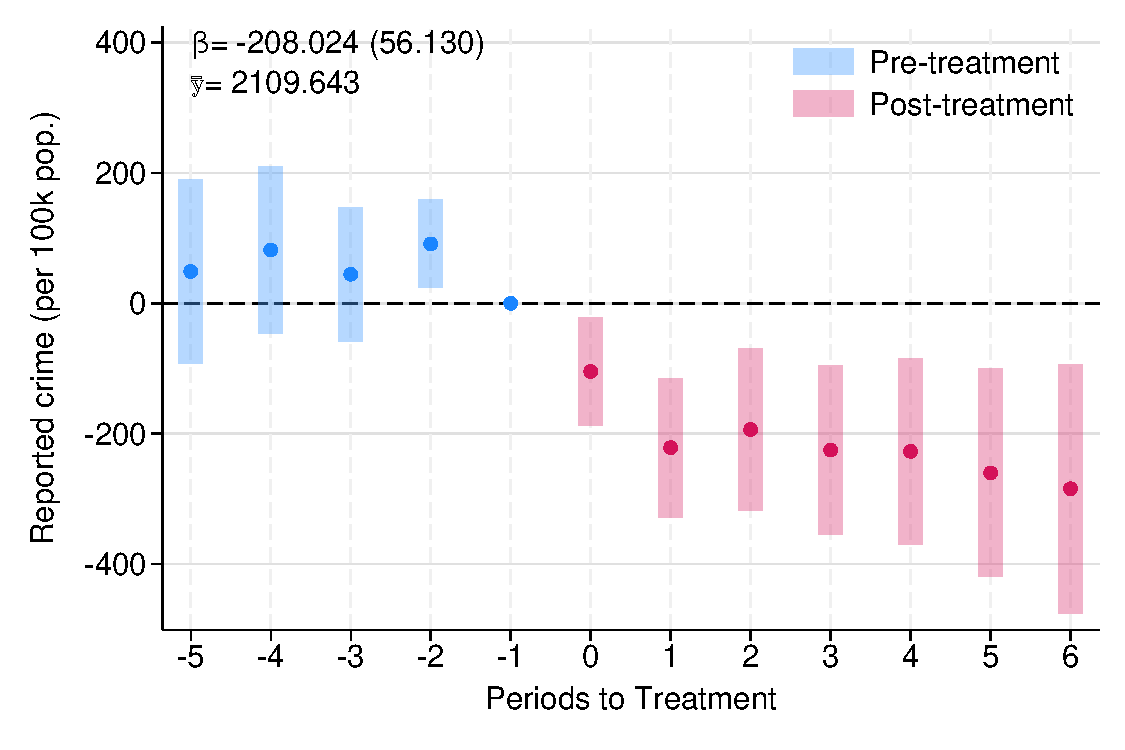
\includegraphics[width=\textwidth]{../manuscript/Graphs/totalreportedcrime_allcomunas.pdf}
        \caption{Reported crime per 100k inhabitants}
    \end{subfigure}
        \begin{subfigure}{0.495\textwidth}
        \centering
        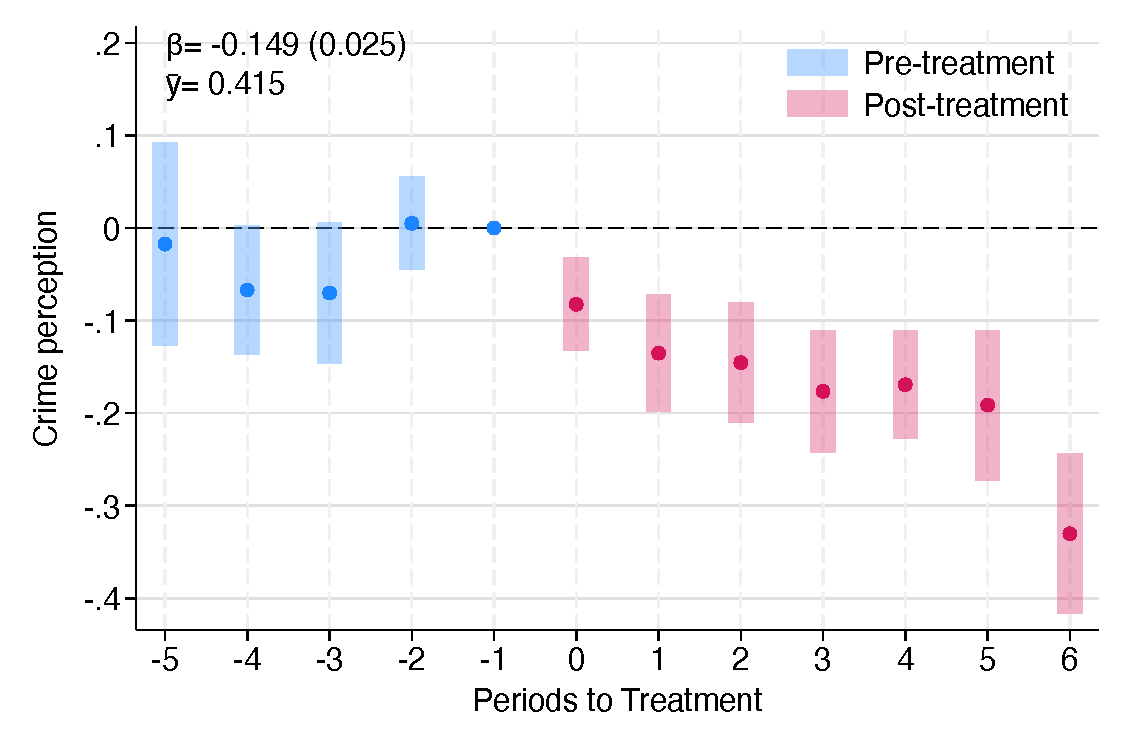
\includegraphics[width=\textwidth]{../manuscript/Graphs/results_perception.pdf}
        \caption{Households reporting an increase in crime}
    \end{subfigure}%
    ~
    \begin{subfigure}{0.495\textwidth}
    \centering
    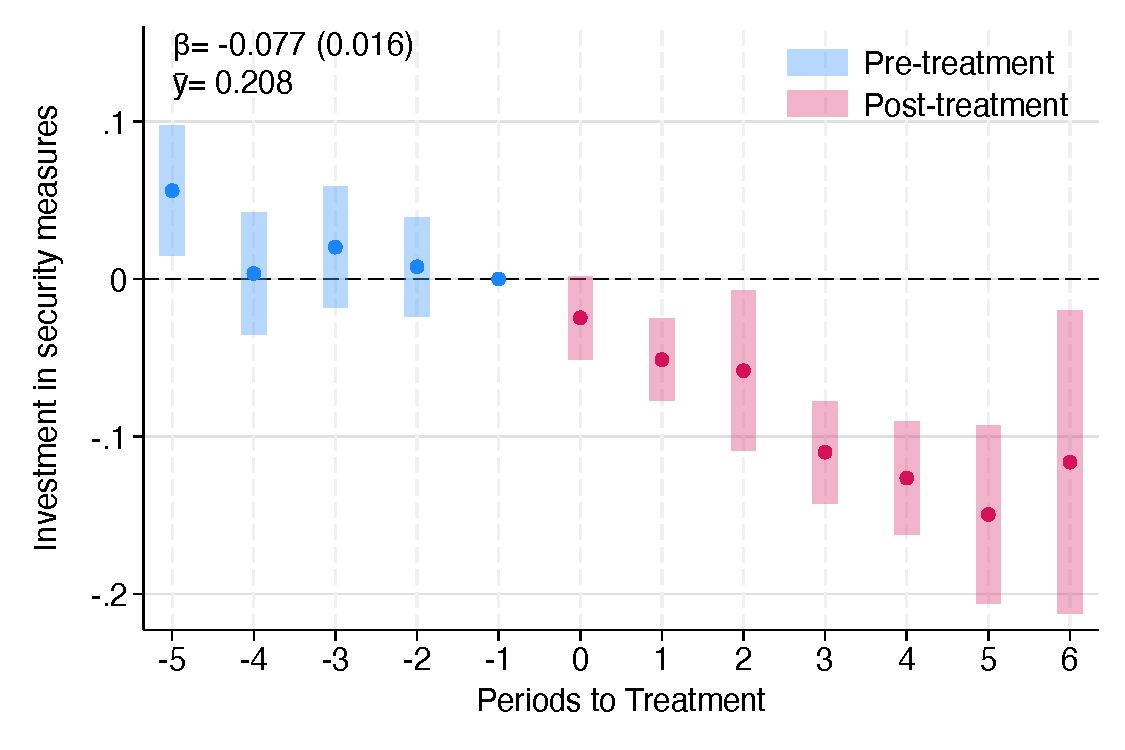
\includegraphics[width=\textwidth]{../manuscript/Graphs/results_hhprotectionmeasures.pdf}
        \caption{Households adopting security measures}
    \end{subfigure}
    \\[12pt]
    \begin{minipage}{0.99\textwidth}
    \footnotesize
    Notes: This figure shows the dynamic effects of the \emph{Plan Cuadrante} on different measures of police effectiveness. The estimation is conducted using the procedure developed in \citet{Callaway} for difference-in-differences with staggered treatment adoption. The dots in the figure represent the estimated coefficients and the bars behind them 95\% confidence intervals. Standard errors are clustered at the municipality level using the wild bootstrapping procedure. The pooled effect and the mean outcome before the introduction of the treatment is also presented in each panel. Panel (a) reports the effect of \emph{Plan Cuadrante} on the probability of household victimization in the last 12 months using the ENUSC survey. Panel (b) reports the effect on the number of crimes reported to the police in the municipality per 100,000 inhabitants using administrative data. Panel (c) reports the effect on the probability of perceiving an increase in crime using the ENUSC survey. Panel (d) reports the effect on the probability of adopting security measures in the last twelve months using the ENUSC survey. Panel (a) includes 93,041 observations; panel (b), 4,231; panel (c), 89,578; and panel (d), 93,041 observations.
    \end{minipage}
\end{figure}
}

\clearpage

{\renewcommand{\thetable}{A.1}
\begin{table}[H]
\centering
\caption{Implementation of \emph{Plan Cuadrante} by Year}
\label{tab:implementation}
\begin{threeparttable}
\begin{tabular}{l c >{\raggedright\arraybackslash}p{10.5cm}}
\toprule
Year & N & Municipalities \\
\midrule
1998--2000 & 44  & Metropolitan Region of Santiago (44 municipalities) \\[3pt]
2002 & 10  & Chiguayante, Concepción, Hualpén, Quilpué, San Antonio, San Pedro de la Paz, Talcahuano, Valparaíso, Villa Alemana, Viña del Mar \\[3pt]
2003 & 2   & Padre Las Casas, Temuco \\[3pt]
2004 & 2   & Antofagasta, Copiapó \\[3pt]
2005 & 7   & Alto Hospicio, Arica, Calama, Curicó, Iquique, Linares, Talca \\[3pt]
2006 & 7   & Coquimbo, La Serena, Los Andes, Ovalle, Rancagua, San Felipe, San Fernando \\[3pt]
2007 & 7   & Chillán, Chillán Viejo, Los Ángeles, Osorno, Puerto Montt, Punta Arenas, Valdivia \\[3pt]
2008 & 9   & Ancud, Castro, Constitución, Coronel, Lota, Peñaflor, Quillota, Rengo, Villarrica \\[3pt]
2009 & 12  & Angol, Aysén, Calera, Concón, Coyhaique, La Unión, Padre Hurtado, Parral, Penco, San Carlos, Tomé, Vallenar \\[3pt]
2011 & 17  & Arauco, Cañete, Cartagena, Cauquenes, Curanilahue, La Ligua, Limache, Molina, Nueva Imperial, Pucón, Puerto Varas, Río Bueno, San Clemente, San Javier, San Vicente, Santa Cruz, Victoria \\[3pt]
2012 & 20  & Cabrero, Calbuco, Casablanca, Chimbarongo, Collipulli, Curacaví, El Monte, Graneros, Illapel, Isla de Maipo, Lautaro, Machalí, Mostazal, Mulchén, Nacimiento, Natales, Panguipulli, Quellón, Quintero, Tocopilla \\[3pt]
2013 & 13  & Bulnes, Laja, Las Cabras, Lebu, Llaillay, Loncoche, Longaví, Los Álamos, Maule, Requínoa, Teno, Vicuña, Yumbel \\
\midrule
Total & 150 & \\
\bottomrule
\end{tabular}
\begin{tablenotes}[flushleft]
\footnotesize
\item Note: \textit{N} is the number of municipalities that adopted \emph{Plan Cuadrante} in each year. Data shared by Carabineros de Chile.
\end{tablenotes}
\end{threeparttable}
\end{table}
}

\clearpage

{\renewcommand{\thefigure}{B.3}
\begin{figure}[h!]
    \centering
    \caption{Effects of \emph{Plan Cuadrante} by Resource Increase: Trust, Complaints, and Arrests}
    \label{fig:heterogeneity_appendix}
    \begin{subfigure}[t]{0.48\textwidth}
        \centering
        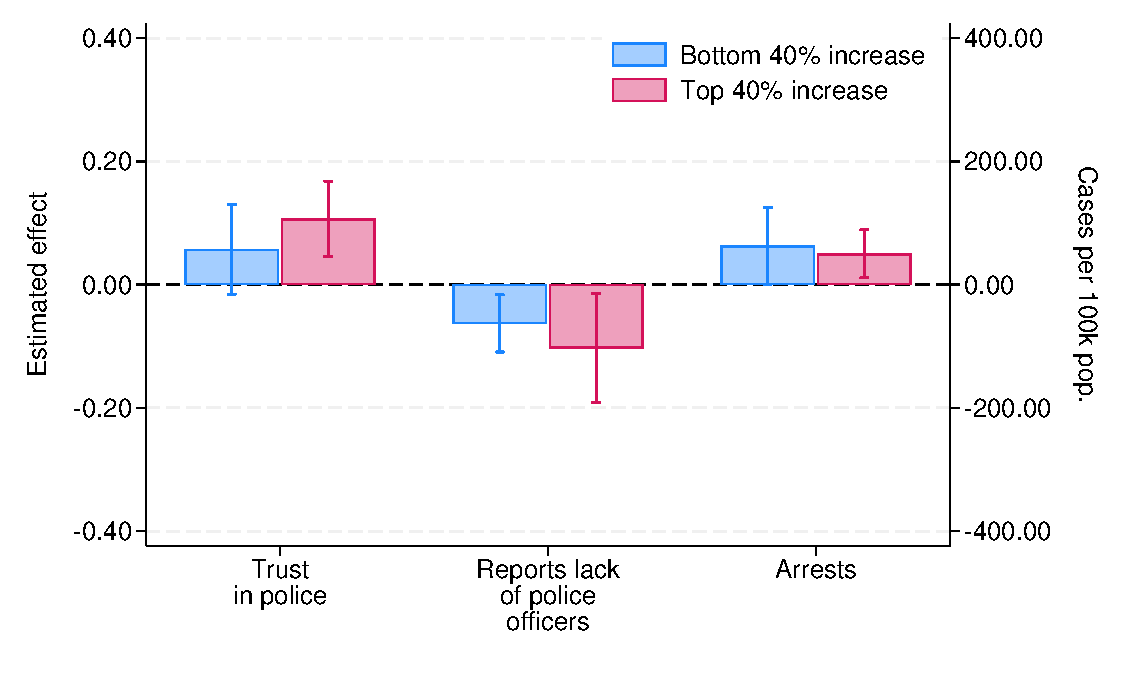
\includegraphics[width=\linewidth]{../manuscript/Graphs/heterogeneity_off_appendix.pdf}
        \caption{By the intensity of $\Delta$ in police officers}
    \end{subfigure}\hfill
    \begin{subfigure}[t]{0.48\textwidth}
        \centering
        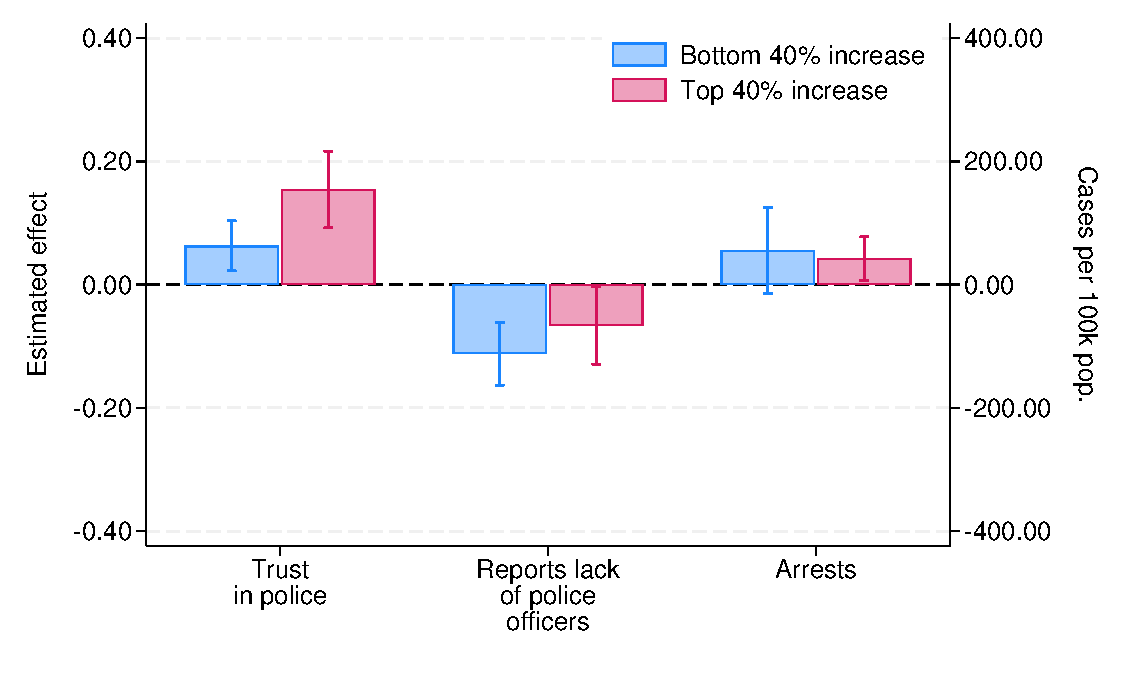
\includegraphics[width=\linewidth]{../manuscript/Graphs/heterogeneity_pv_appendix.pdf}
        \caption{By the intensity of $\Delta$ in patrol vehicles}
    \end{subfigure}
    \\[8pt]
    \begin{minipage}{0.99\textwidth}
    \footnotesize Notes: This figure complements Figure \ref{fig:figure_resources} by reporting, for the three outcomes not shown there, the effect of \emph{Plan Cuadrante} estimated separately for municipalities in the bottom 40\% (blue) and top 40\% (red) of the resource-increase distribution. Panel (a) splits municipalities by the increase in police officers and panel (b) by the increase in patrol vehicles. In each panel, arrests (administrative data, in cases per 100,000 inhabitants) are read on the right axis; the other two outcomes, from the ENUSC survey (trust in the police, and reports about the lack of police officers), are read on the left axis. Effects are estimated using the difference-in-differences estimator for staggered treatment adoption developed in \citet{Callaway}; bars are point estimates and whiskers 95\% confidence intervals, with standard errors clustered at the municipality level using the wild bootstrapping procedure.
    \end{minipage}
\end{figure}
}

\clearpage

{\renewcommand{\thetable}{B.3}
\begin{table}[h!]\centering
\caption{Effects of \emph{Plan Cuadrante} Controlling for Police Resources}
\label{tab:results_controlbyresources}
\resizebox{\textwidth}{!}{
\begin{threeparttable}
\begin{tabular}{l ccccc}
\toprule
 & (1) & (2) & (3) & (4) & (5) \\
\midrule
\multicolumn{6}{l}{\textit{Panel A. Victimization}} \\[0.2em]
ATT &       -0.099*** &       -0.077*** &       -0.086** &       -0.094*** &       -0.087* \\
  & (0.013) & (0.013) & (0.043) & (0.028) & (0.053) \\
N &    93,041 &    53,973 &    53,553 &    72,017 &    53,553 \\[0.4em]
\multicolumn{6}{l}{\textit{Panel B. Crime perception}} \\[0.2em]
ATT &       -0.149*** &       -0.140*** &       -0.112** &       -0.082** &       -0.111 \\
  & (0.025) & (0.032) & (0.057) & (0.033) & (0.106) \\
N &    89,578 &    52,160 &    51,746 &    69,434 &    51,746 \\[0.4em]
\multicolumn{6}{l}{\textit{Panel C. Investment in security measures}} \\[0.2em]
ATT &       -0.077*** &       -0.066*** &       -0.109*** &       -0.081*** &       -0.168*** \\
  & (0.016) & (0.019) & (0.041) & (0.019) & (0.064) \\
N &    93,041 &    53,973 &    53,553 &    72,017 &    53,553 \\[0.4em]
\multicolumn{6}{l}{\textit{Panel D. Reported crime (per 100k pop.)}} \\[0.2em]
ATT &     -208.024*** &     -190.446*** &       29.230 &     -261.439 &     -245.555 \\
  & (56.130) & (67.908) & (147.261) & (170.954) & (165.221) \\
N &     4,231 &     1,918 &     1,911 &     2,248 &     1,911 \\[0.4em]
\midrule
Sample                   & Full & Resource yrs & Resource yrs & Resource yrs & Resource yrs \\
Police officers (per 100k pop.) &      &            & \checkmark &            & \checkmark \\
Patrol vehicles (per 100k pop.) &      &            &            & \checkmark & \checkmark \\
\bottomrule
\end{tabular}
\begin{tablenotes}[flushleft]
\item \footnotesize{Note: ATT estimates of the effect of \emph{Plan Cuadrante} on each outcome. Column (1) is the baseline (full estimation sample, no controls) and reproduces the headline estimate of the corresponding estimator. Column (2) restricts the estimation to 2006--2012, the window over which police resources are observed, without including any control variable. Columns (3)--(5) add time-varying controls for police resources per 100{,}000 inhabitants: officers only; patrol vehicles only; and officers and patrol vehicles jointly (entered as separate regressors). Columns (3) and (5) cover 2006--2012, the years for which the number of officers is observed; column (4) also includes 2005, the first year for which patrol vehicles are observed. Patrol vehicles are measured, per 100{,}000 inhabitants, as all patrol automobiles (radiopatrulla, auto patrullero, auto policial, automovil, station wagon, jeep and camioneta) plus motorcycles. Standard errors in parentheses; row N reports the estimation-sample size. Estimation follows \citet{Callaway}; standard errors clustered at the municipality level using wild bootstrapping procedures. $^{*}p<0.1$, $^{**}p<0.05$, $^{***}p<0.01$.}
\end{tablenotes}
\end{threeparttable}}
\end{table}
}

\clearpage

{\renewcommand{\thefigure}{B.4}
\begin{figure}[h!]
    \centering
    \caption{Effects of \textit{Seguridad Ciudadana} on Crime Outcomes and Security Perceptions}
    \label{fig:figureA5}
    
    % Primera fila: panel (a) y (b)
    \begin{subfigure}{0.495\textwidth}
        \centering
        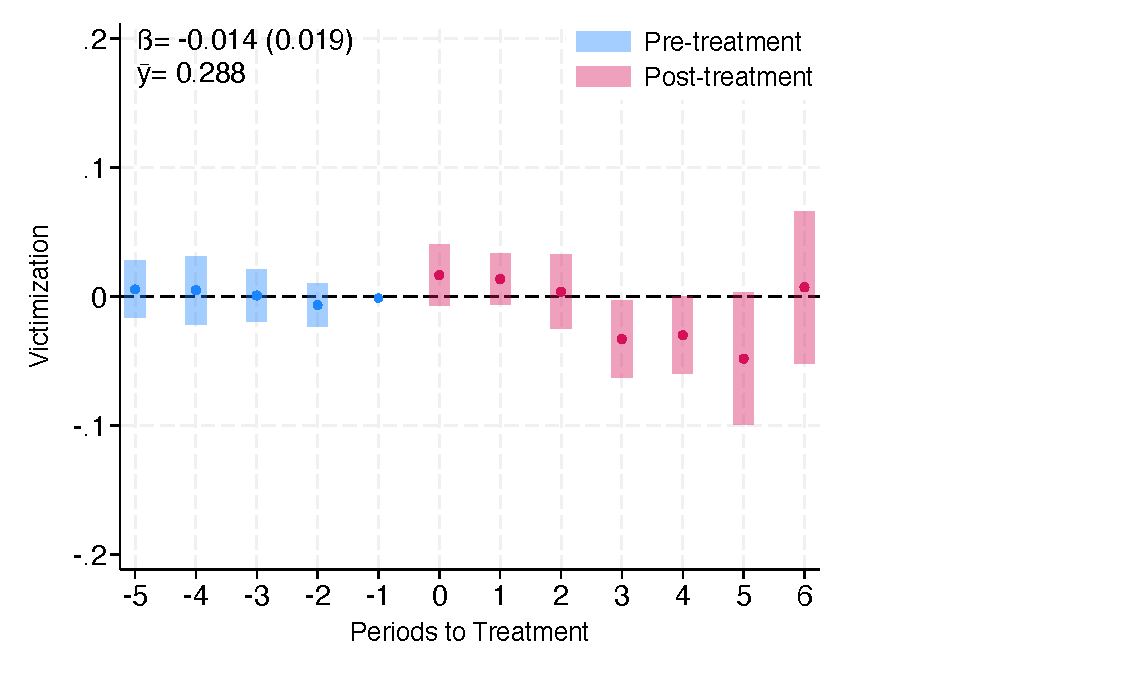
\includegraphics[width=\textwidth]{../manuscript/Graphs/results_victimization_SC.pdf}
        \caption{Victimization in last 12 months}
    \end{subfigure}%
    \hfill
    \begin{subfigure}{0.495\textwidth}
        \centering
        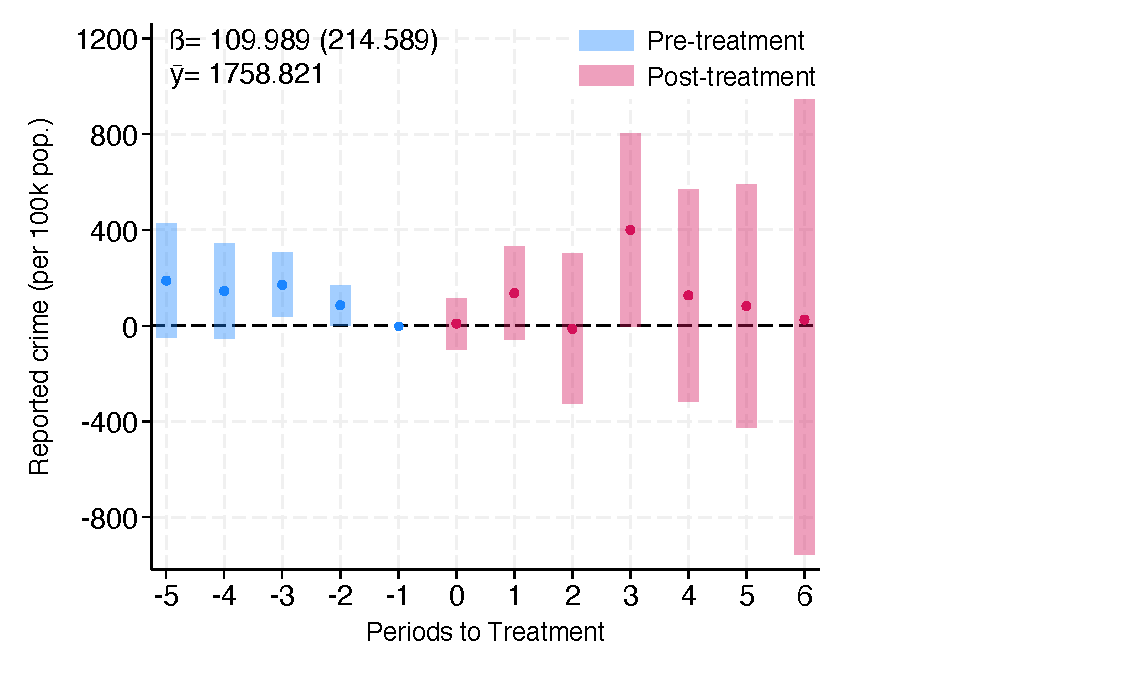
\includegraphics[width=\textwidth]{../manuscript/Graphs/totalreportedcrime_allcomunas_SC.pdf}
        \caption{Reported crime per 100k inhabitants}
    \end{subfigure}

    \vspace{12pt} % Espacio entre filas
    
    % Segunda fila: panel (c) y (d)
    \begin{subfigure}{0.495\textwidth}
        \centering
        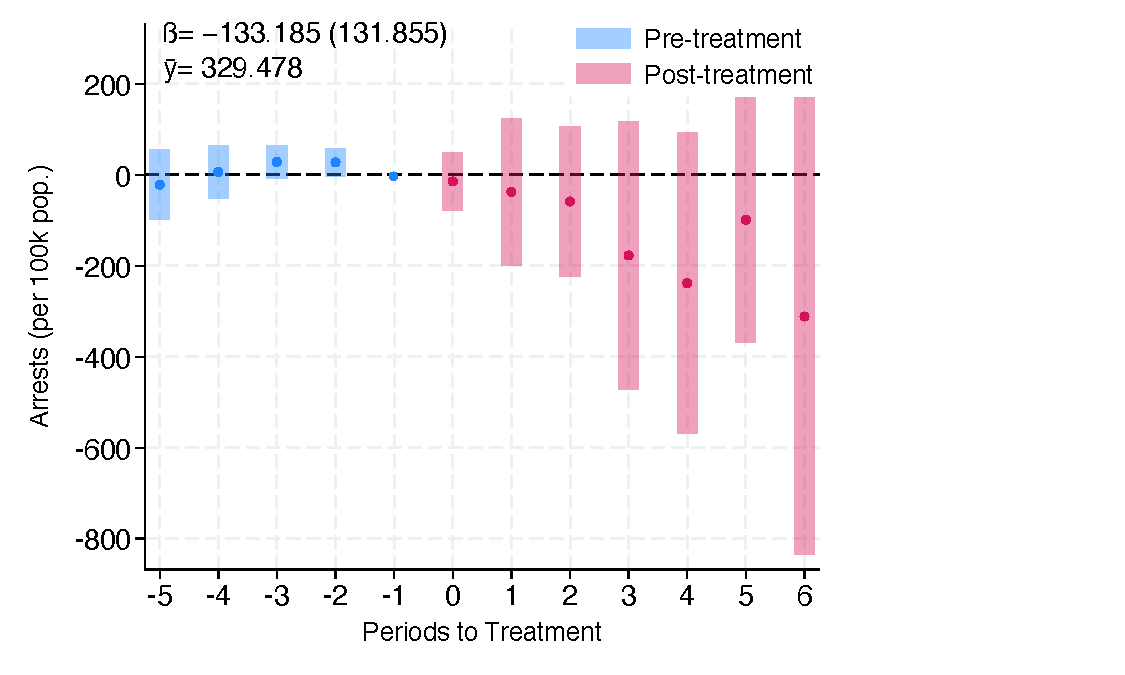
\includegraphics[width=\textwidth]{../manuscript/Graphs/totalarrestscrime_allcomunas_SC.pdf}
        \caption{Arrests per 100k inhabitants}
    \end{subfigure}%
    \hfill
    \begin{subfigure}{0.495\textwidth}
        \centering
        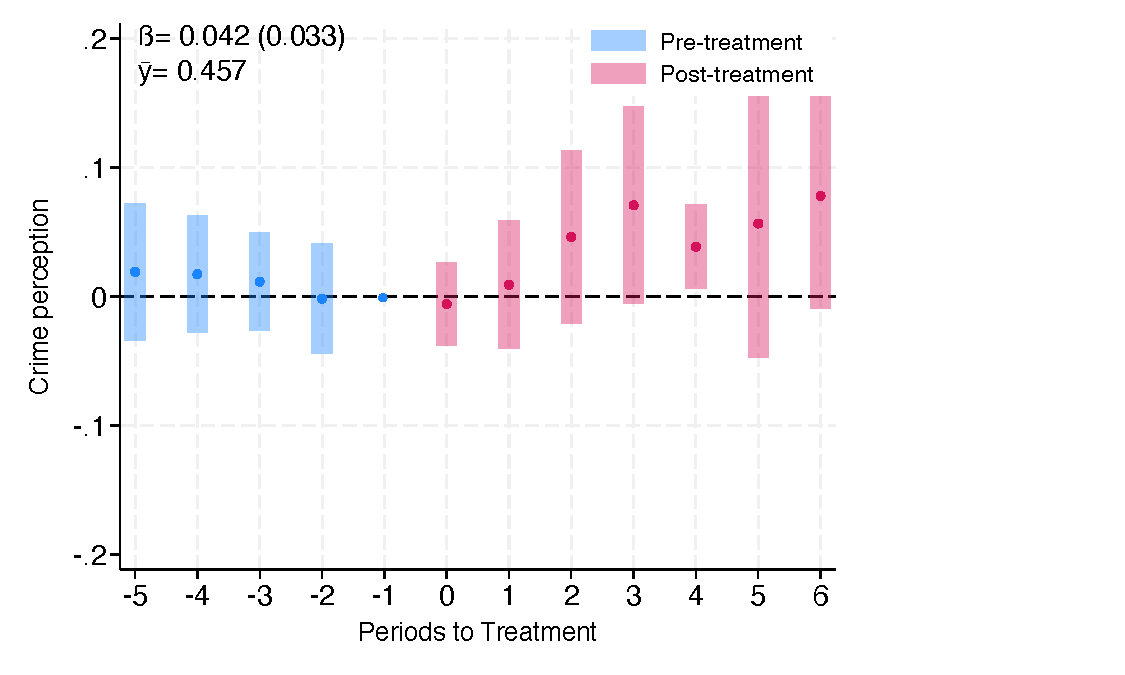
\includegraphics[width=\textwidth]{../manuscript/Graphs/results_perception_SC.pdf}
        \caption{Households reporting an \\ increase in crime}
    \end{subfigure}
    
    \vspace{12pt} % Espacio entre filas
    
    % Tercera fila: panel (e)
    \begin{subfigure}{0.495\textwidth}
        \centering
        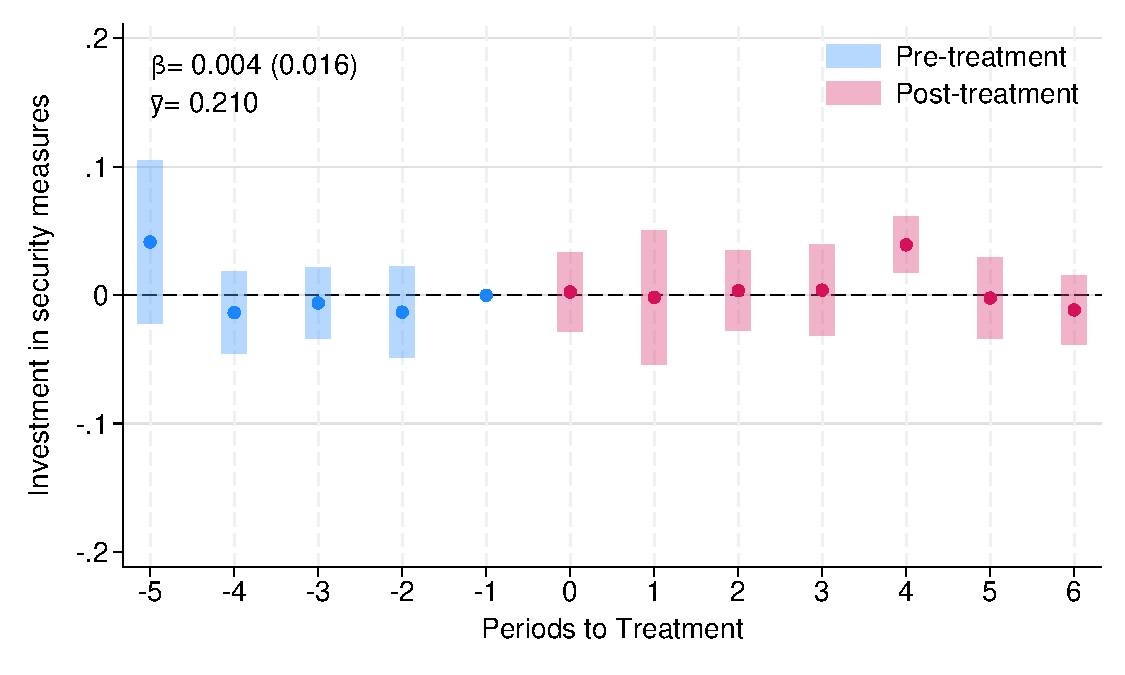
\includegraphics[width=\textwidth]{../manuscript/Graphs/results_hhprotectionmeasures_SC.pdf}
        \caption{Households adopting security measures}
    \end{subfigure}

    \vspace{12pt} % Espacio para las notas
    
    \begin{minipage}{0.99\textwidth}
        \footnotesize
        Notes: This figure shows the dynamic effects of the \textit{Seguridad Ciudadana} program on different measures of crime and security perceptions. The estimation is conducted using the procedure developed in \citet{Callaway} for difference-in-differences with staggered treatment adoption. The dots in the figure represent the estimated coefficients and the bars behind them 95\% confidence intervals. Standard errors are clustered at the municipality level using wild bootstrapping. The pooled effect and the mean outcome before the introduction of the treatment for the outcome---computed as in Figure \ref{fig:figure02}, using only the pre-treatment observations of treated units---is also presented in each panel. Panel (a) reports the effect of \textit{Seguridad Ciudadana} on the probability of household victimization in the last 12 months using the ENUSC survey. Panel (b) reports the effect on the number of crimes reported to the police in the municipality per 100,000 inhabitants using administrative data. Panel (c) reports the effect on the number of arrests in the municipality per 100,000 inhabitants using administrative data. Panel (d) reports the effect on the probability of perceiving an increase in crime using the ENUSC survey. Panel (e) reports the effect on the probability of adopting security measures in the last twelve months using the ENUSC survey. Panel (a) includes 210,102 observations; panel (b), 2,234; panel (c), 1,908; panel (d), 203,078; and panel (e), 74,316 observations.
    \end{minipage}
\end{figure}
}

\clearpage

{\renewcommand{\thefigure}{B.5}
\begin{figure}[h!]
    \centering
    \caption{Association between Police Resources and Police Effectiveness (No \emph{Plan Cuadrante} Variation)}
    \label{fig:figureA7B}
    \begin{subfigure}[t]{0.48\textwidth}
        \centering
        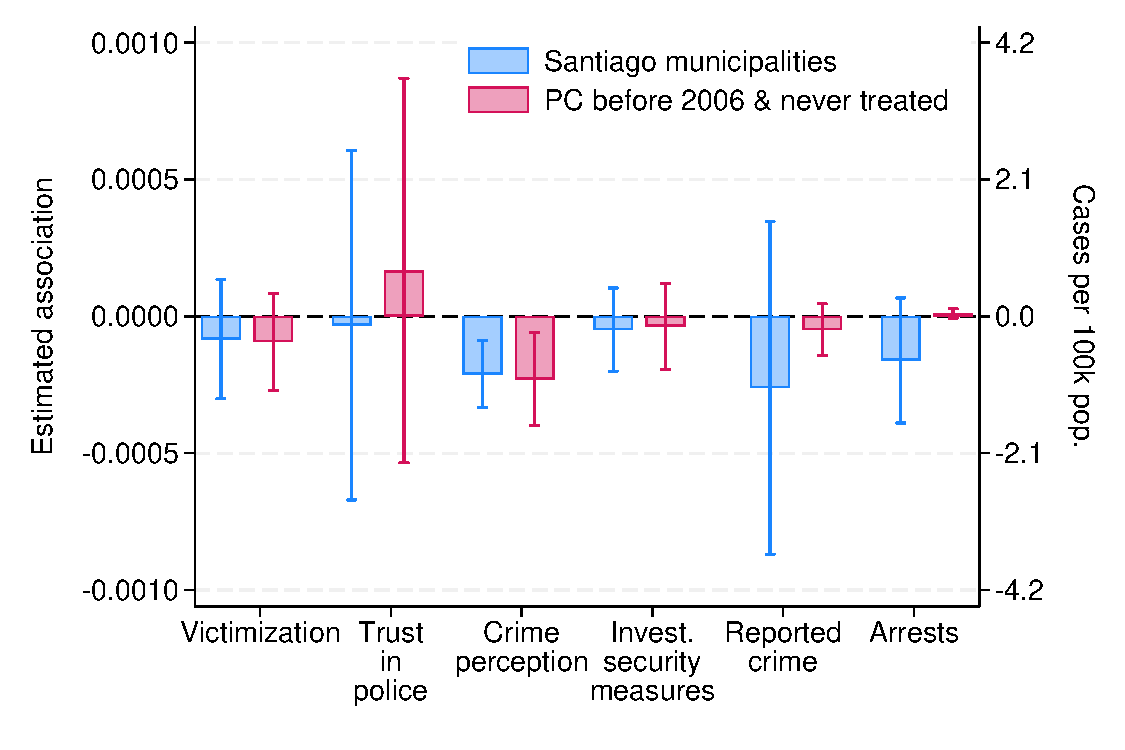
\includegraphics[width=\linewidth]{../manuscript/Graphs/results_corr_novariation_off.pdf}
        \caption{Association with police officers}
    \end{subfigure}\hfill
    \begin{subfigure}[t]{0.48\textwidth}
        \centering
        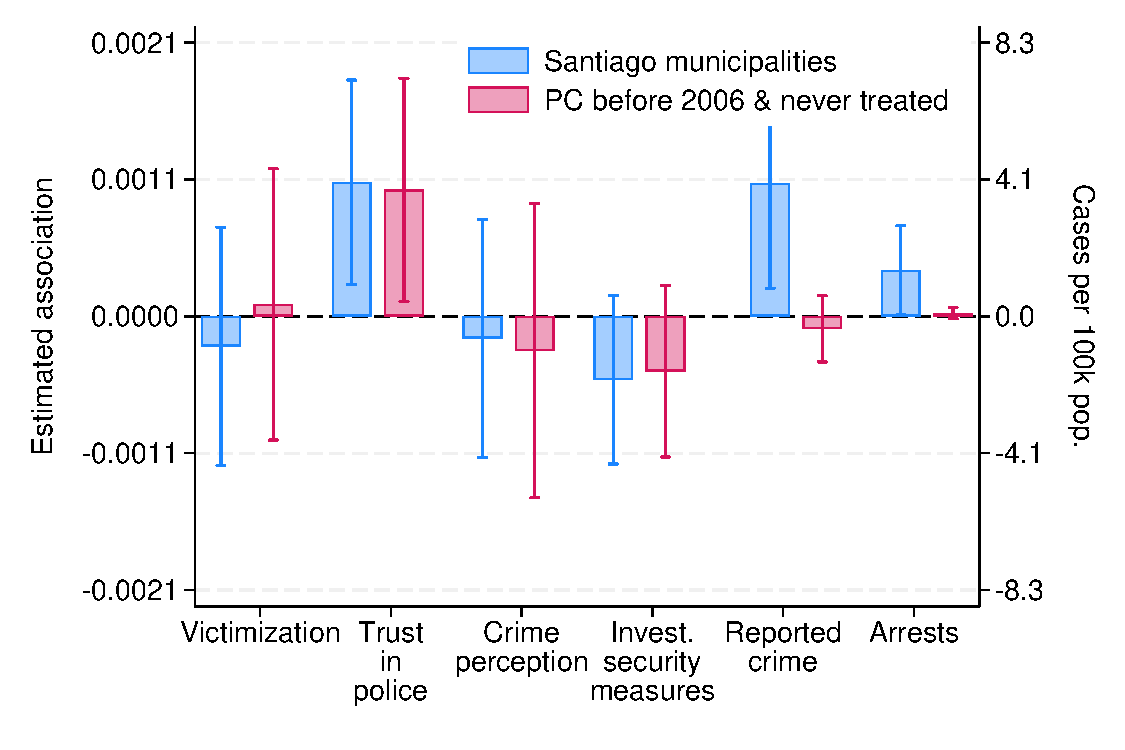
\includegraphics[width=\linewidth]{../manuscript/Graphs/results_corr_novariation_veh.pdf}
        \caption{Association with patrol vehicles}
    \end{subfigure}
    \\[10pt]
    \begin{minipage}{0.99\textwidth}
    \footnotesize Notes: The figure shows the estimated within-municipality association between police resources (per 100,000 inhabitants) and the main outcomes, in municipalities where \emph{Plan Cuadrante} does not vary over the sample period. Estimates come from OLS regressions of each outcome on the resource measure with municipality and year fixed effects; standard errors are clustered at the municipality level. Blue bars use the 41 metropolitan municipalities of Santiago, all of which adopted \emph{Plan Cuadrante} in 2000; red bars use the broader set of municipalities that adopted \emph{Plan Cuadrante} before 2006 together with the never-treated municipalities surveyed in ENUSC (2006--2012). Reported crime and arrests (administrative data, in cases per 100,000 inhabitants) are read on the right axis; all other outcomes, from the ENUSC survey (victimization, trust in the police, crime perception, and investment in security measures), are read on the left axis. Panel (a) reports associations with the number of police officers; panel (b) with the number of patrol vehicles. Bars are point estimates with 95\% confidence intervals.
    \end{minipage}
\end{figure}
}

\clearpage

{\renewcommand{\thetable}{B.4}
\begin{table}[H]
\centering
\caption{Predictors of the Increase in Police Resources under \emph{Plan Cuadrante}}
\label{tab:resourcecorrelates}
\begin{threeparttable}
\small
\setlength{\tabcolsep}{6pt}
\renewcommand{\arraystretch}{1.1}
\begin{tabular}{@{}l cc cc@{}}
\toprule
& \multicolumn{2}{c}{Administrative sample} & \multicolumn{2}{c}{ENUSC sample} \\
\cmidrule(lr){2-3} \cmidrule(lr){4-5}
& Police & Patrol & Police & Patrol \\
Dep.\ var: avg.\ annual increase & officers & vehicles & officers & vehicles \\
in resources (share of pre-adoption level) & (1) & (2) & (3) & (4) \\
\midrule
Reported crime (per 100k pop.) & $-0.203^{**}$ & $-0.199^{**}$ & $-0.319^{*}$ & $0.272^{*}$ \\
 & (0.099) & (0.097) & (0.182) & (0.137) \\
Arrests (per 100k pop.) & $0.099$ & $-0.041$ & $0.003$ & $0.297$ \\
 & (0.136) & (0.129) & (0.186) & (0.223) \\
Victimization &  &  & $-0.017^{*}$ & $-0.025^{*}$ \\
 &  &  & (0.010) & (0.013) \\
Crime perception &  &  & $0.005$ & $0.008$ \\
 &  &  & (0.017) & (0.014) \\
Trust in the police &  &  & $0.024$ & $0.027$ \\
 &  &  & (0.018) & (0.019) \\
Investment in security measures &  &  & $0.004$ & $-0.003$ \\
 &  &  & (0.010) & (0.009) \\
Police officers (per 100k pop.) & $-0.207$ & $0.155$ & $-0.888^{***}$ & $0.571^{***}$ \\
 & (0.155) & (0.129) & (0.154) & (0.136) \\
Patrol vehicles (per 100k pop.) & $-0.129$ & $-0.139$ & $0.537^{**}$ & $-0.507^{***}$ \\
 & (0.129) & (0.126) & (0.212) & (0.169) \\
Log population & $-0.529^{***}$ & $-0.203^{*}$ & $-0.193$ & $-0.626^{**}$ \\
 & (0.145) & (0.112) & (0.189) & (0.269) \\
Poverty rate (2004) & $0.170$ & $0.308^{**}$ & $0.027$ & $-0.017$ \\
 & (0.113) & (0.126) & (0.108) & (0.108) \\
\midrule
Observations & 65 & 65 & 8,781 & 8,781 \\
R-squared & 0.342 & 0.282 & 0.614 & 0.545 \\
\bottomrule
\end{tabular}
\begin{tablenotes}[flushleft]
\footnotesize
\item \textit{Note:} OLS regressions of the average annual increase in police officers (columns 1 and 3) and patrol vehicles (columns 2 and 4) per 100{,}000 inhabitants, from the year before adoption of \emph{Plan Cuadrante} to 2012. As in panels (a) and (b) of Figure \ref{fig:figure_resources}, the increase is expressed as a share of the resources available the year before adoption. Columns 1--2 use the administrative sample at the municipality level; columns 3--4 use ENUSC survey respondents interviewed before 2007 (survey outcomes at the respondent level, other regressors as pre-2006 municipality aggregates). All variables are standardized. Standard errors clustered by municipality in parentheses.
\item $^{*}p<0.1$; $^{**}p<0.05$; $^{***}p<0.01$.
\end{tablenotes}
\end{threeparttable}
\end{table}
}

\clearpage

{\renewcommand{\thefigure}{B.6}
\begin{figure}[H]
    \centering
    \caption{Timing of Adoption of \emph{Plan Cuadrante} and Perceived Police Performance}
    \label{fig:balance_doseresponse}
    \begin{subfigure}{0.495\textwidth}
        \centering
        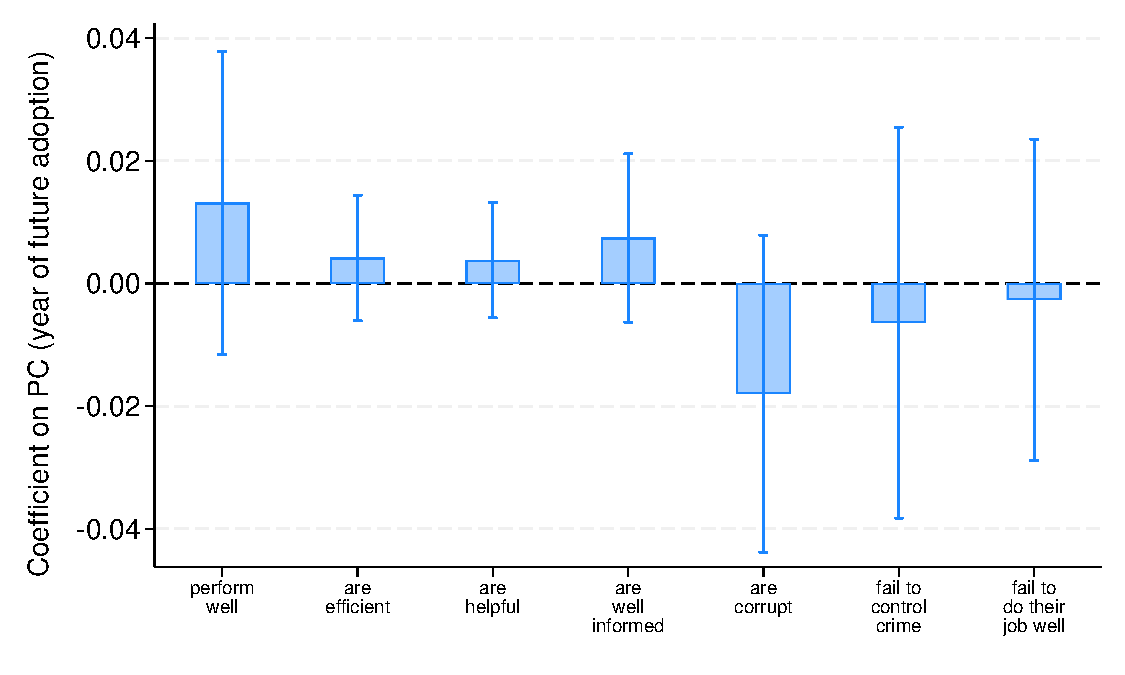
\includegraphics[width=\textwidth]{../manuscript/Graphs/balance_carabperc.pdf}
        \caption{Year of adoption and police performance before adoption}
    \end{subfigure}%
    ~
    \begin{subfigure}{0.495\textwidth}
        \centering
        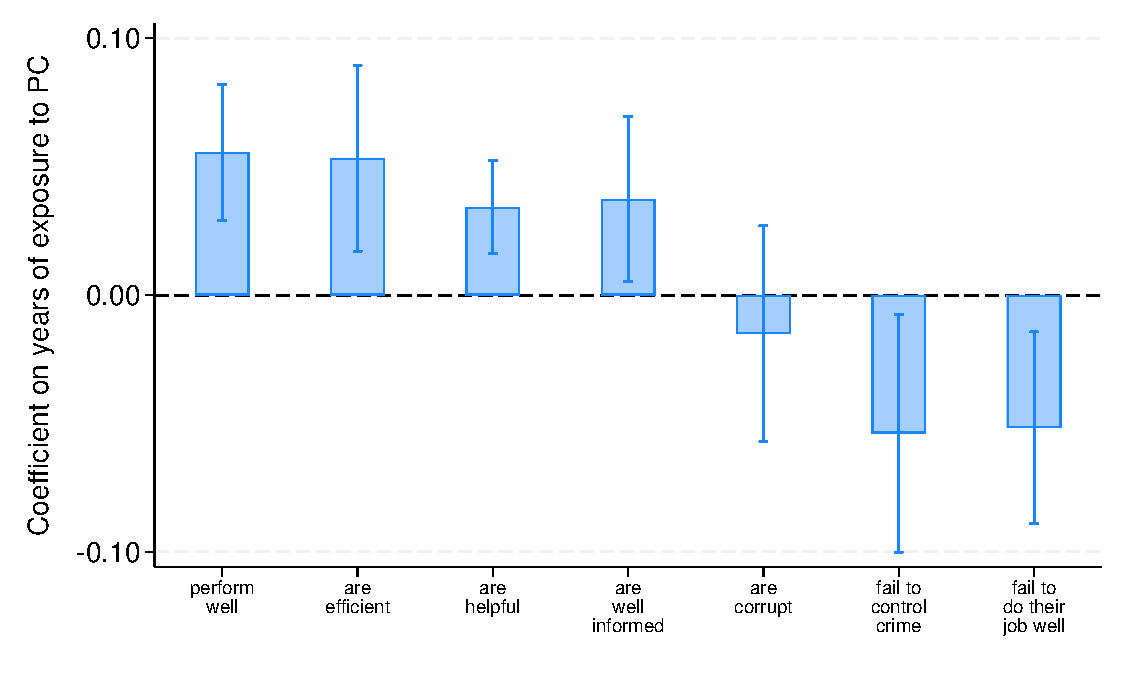
\includegraphics[width=\textwidth]{../manuscript/Graphs/doseresponse_carabperc.pdf}
        \caption{Years exposed to \emph{Plan Cuadrante} (dose response)}
    \end{subfigure}%
    \\[12pt]
    \begin{minipage}{0.99\textwidth}
    Notes: The figure considers seven measures of police performance: the share of respondents who perceive police performance as good, and who perceive the police to be efficient, helpful, well informed, corrupt, failing to control crime, and failing to do their job well. Using the sample of municipalities that adopted \emph{Plan Cuadrante} after 2005, panel (a) examines whether the future timing of adoption of \emph{Plan Cuadrante} is correlated with perceived police performance in 2005, before the introduction of the program. Panel (b) reestimates the same comparison as Figure \ref{fig:figure05}, replacing the binary adoption indicator with the municipality's number of years of exposure to \emph{Plan Cuadrante} as of 2005. In both panels, each bar plots the coefficient from a separate regression of one performance measure. The graphs display the estimated coefficients and 95\% confidence intervals.
    \end{minipage}
\end{figure}
}

\clearpage

{\renewcommand{\thefigure}{C.8}
\begin{figure}[h!]
    \centering
    \caption{Effects of \emph{Plan Cuadrante} on Reported Crime and Arrests Using the Full Set of Post-treatment and Pre-treatment Periods}
    \label{fig:admin_uncapped}
    \begin{subfigure}{0.495\textwidth}
        \centering
        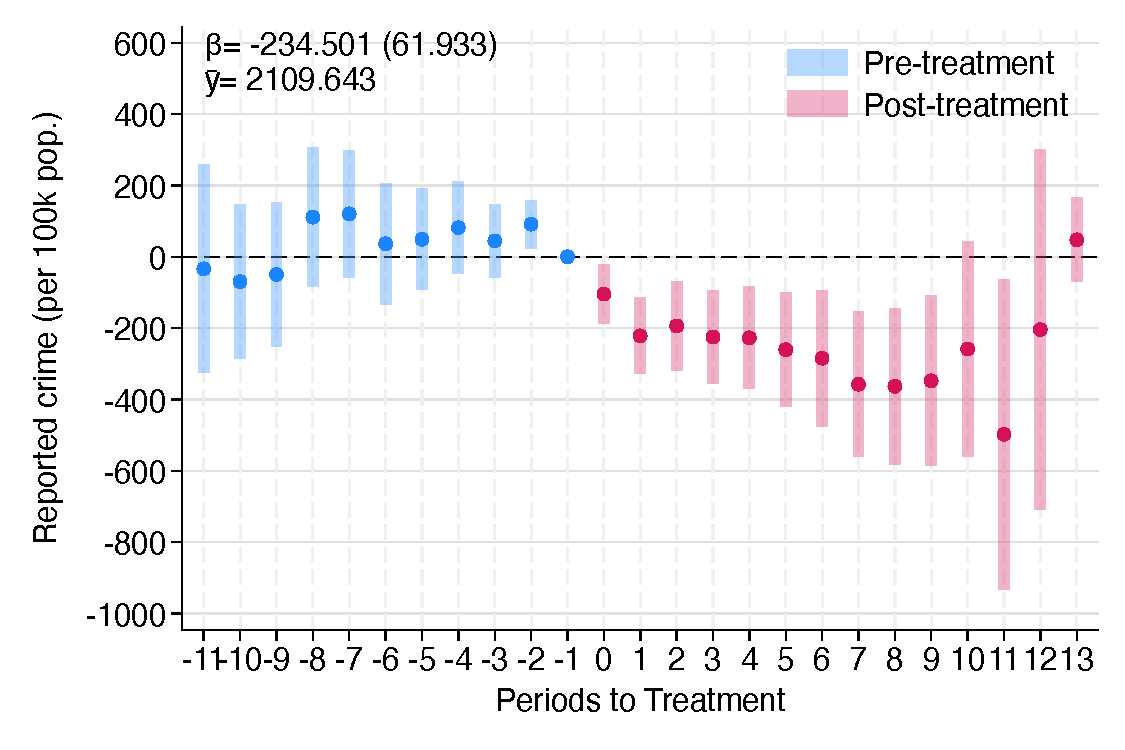
\includegraphics[width=0.98\textwidth]{../manuscript/Graphs/totalreportedcrime_allcomunas_uncapped.pdf}
        \caption{Reported crime per 100k inhabitants}
    \end{subfigure}%
    ~
    \begin{subfigure}{0.495\textwidth}
    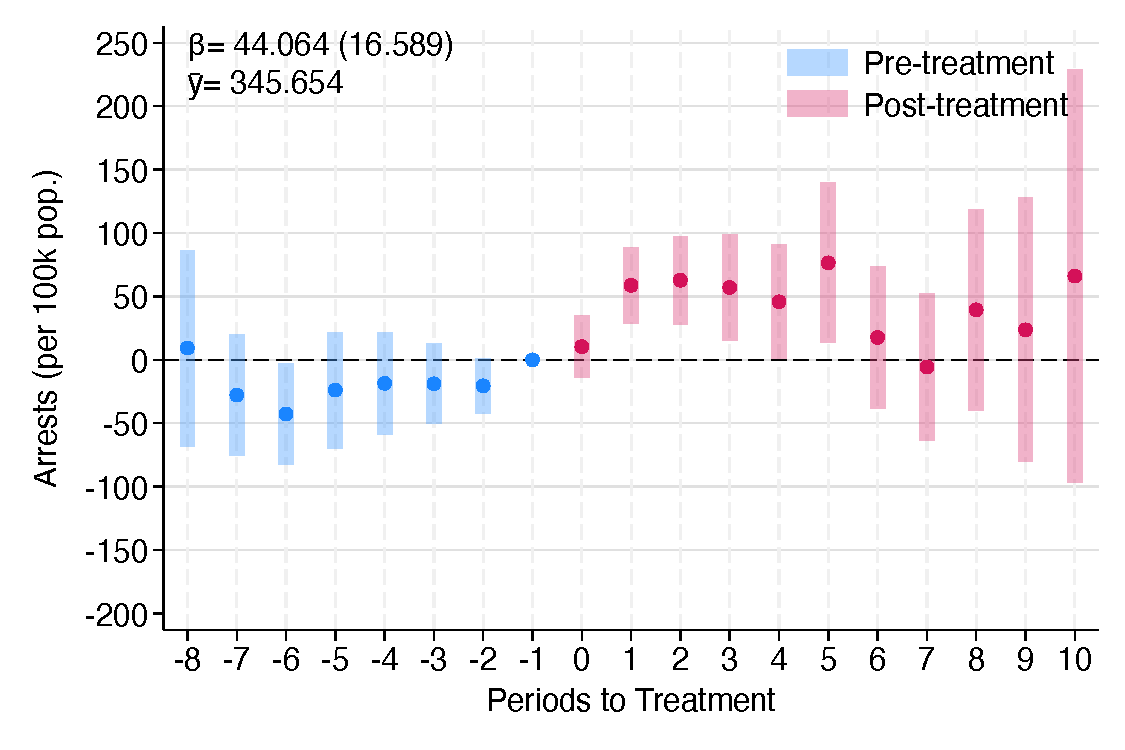
\includegraphics[width=0.98\textwidth]{../manuscript/Graphs/totalarrestscrime_allcomunas_uncapped.pdf}
        \caption{Arrests per 100k inhabitants}
    \end{subfigure}
    \begin{minipage}{\textwidth}
    \footnotesize
   Notes: This figure shows the dynamic effects of \emph{Plan Cuadrante} on the number of crimes reported to the police in the municipality per 100,000 inhabitants (panel a) and on the number of arrests in the municipality per 100,000 inhabitants (panel b), using administrative data. The estimation is conducted using the procedure developed in \citet{Callaway} for difference-in-differences with staggered treatment adoption. The dots in the figure represent the estimated coefficients and the bars behind them 95\% confidence intervals. Standard errors are clustered at the municipality level using the wild bootstrapping procedure. The pooled effect and the mean outcome before the introduction of the treatment are also presented in each panel. Unlike Figure \ref{fig:figure02} in the main text, we do not cap the event study to the same 5 pre-treatment and 6 post-treatment periods used for symmetry with the ENUSC-based analysis. Instead, we exploit the full set of post-treatment and pre-treatment periods. Panel (a) includes 4,371 observations and panel (b) 3,372 observations.
    \end{minipage}
\end{figure}
}

\clearpage

\end{editorresponse}
\stepcounter{AnsweredComments}


%\begin{editorcomment}
%After I receive your revised manuscript and replies, I will assess the progress made on the points raised by the reviewers and send the paper back to them. While there is no strict deadline for this revision, I would hope that you can return a revised manuscript within three months. Please let me know if you encounter any issues with this timeline or if anything in my letter or in the reports is unclear.
%\\[6pt]
%Thank you again for giving me the opportunity to read your excellent paper. I look forward to seeing the revised version.
%\\[6pt]
%Best,
%\\[6pt]
%Roland Rathelot
%\end{editorcomment}

\putbib
\end{bibunit}
